% Seminar deck v4 (business-school version; v3 plus David's slide-by-slide edits of 2026-10-03, see deck_v3_david_edits.md; v3 frozen): "Refusing to concede? War and everyday rivalry online"
% 45-minute economics seminar. Source of truth for every number: docs/prose_drafts/full_draft_v4_2.md
% and the frozen number manifest (data freeze 2b6d3f3). Figures: seminar/figures/make_slide_figures.py.
%
% Single variant: Next Steps carries the Iran preregistered replication (the former variant A).
\documentclass[aspectratio=169,11pt,t]{beamer}
\usetheme{default}
\usecolortheme{dove}
\usepackage[T1]{fontenc}
\usepackage[utf8]{inputenc}
\usepackage{lmodern}
\usepackage{amsmath}
\usepackage{booktabs}
\usepackage{array}
\usepackage{graphicx}
\usepackage{tikz}
\usepackage{hyperref}

\graphicspath{{figures/out/}{figures/source/}}

\setbeamertemplate{navigation symbols}{}
\setbeamertemplate{footline}{%
  \hfill{\scriptsize\textcolor{gray}{\insertframenumber}}\hspace{4mm}\vspace{2mm}}
\setbeamertemplate{itemize items}[circle]
\setbeamertemplate{enumerate items}[default]
\setbeamerfont{frametitle}{size=\large,series=\bfseries}
\setbeamerfont{block title}{series=\bfseries}
\setbeamercolor{block title}{bg=black!8,fg=black}
\setbeamercolor{block body}{bg=black!3}
\setbeamersize{text margin left=8mm,text margin right=8mm}
\setlength{\leftmargini}{1.4em}

\definecolor{rawblue}{HTML}{2A78D6}
\definecolor{engorange}{HTML}{EB6834}
\definecolor{linkblue}{HTML}{1F5FAD}
\hypersetup{colorlinks=true,linkcolor=linkblue,urlcolor=linkblue}

% small coloured cross-reference links
\newcommand{\bk}[2]{\hyperlink{#1}{\textcolor{linkblue}{\scriptsize\textsf{backup: #2}}}}
\newcommand{\fq}[2]{\hyperlink{#1}{\textcolor{linkblue}{\scriptsize\textsf{FAQ: #2}}}}
\newcommand{\backto}[2]{\vfill\hfill\hyperlink{#1}{\textcolor{linkblue}{\scriptsize\textsf{back: #2}}}}
\newcommand{\links}[1]{\vfill\hfill{#1}}
\newcommand{\src}[1]{{\vfill\scriptsize\textcolor{gray}{#1}}}
\newcommand{\pp}{pp}

\title{Refusing to concede? War and everyday rivalry online}
\author{David Smerdon}
\institute{University of Queensland}


\begin{document}

% =====================================================================
% 1. TITLE
% =====================================================================
\begin{frame}[plain]
  \vspace{16mm}
  \begin{center}
    {\LARGE\bfseries Refusing to concede?}\\[2mm]
    {\Large\bfseries War and everyday rivalry online}\\[14mm]
    {\large David Smerdon}\\[5mm]
    {\normalsize (with Eren Bilen, Nino Doghonadze, Robizon Khubulashvili)}\\[2mm]
    {\normalsize University of Queensland}
  \end{center}
\end{frame}

% =====================================================================
% MOTIVATION
% =====================================================================
\section{Motivation}

\begin{frame}[label=motivation]{Concession and the cost of continuing}
  \footnotesize
  \begin{itemize}
    \item A dispute ends only when someone accepts an end to it: a settlement, a renegotiated loan, a disputed invoice paid or written off
    \item Not conceding is costly. In wholesale vehicle negotiations, failed trades destroy an estimated 12--23\% of the available gains from trade (Larsen 2021); most long-term credit agreements are renegotiated before maturity (Roberts and Sufi 2009); after 2014, Russian courts enforced fewer foreign claims (Shchetinin and Avdeev 2026)
    \item These studies are evidence of the downstream effect on applications, but little is known about the fundamental decision process underneath.     \item Online chess records the concession decision in its simplest form: a unilateral concession, one click, directed at one identifiable opponent, in 32.4 million games
  \end{itemize}
  \small
  \begin{block}{}
    \centering
    When wars begin, do individuals change how they treat members of the opposing country in everyday encounters that have nothing to do with the war?
  \end{block}
  \links{\bk{bk-lit1}{literature: conflict} \quad \bk{bk-lit2}{literature: markets}}
\end{frame}

\begin{frame}[label=whychess]{Why chess?}
  \begin{itemize}
    \item People play online chess every day against strangers whom the platform pairs with them; each opponent's displayed country is visible before the first move; the encounter has nothing to do with the war
    \item The same individuals meet counterparts from the other side both before a war begins and after, far from the battlefield. Few settings record such meetings at all; online chess records every one
    \item Every game leaves a complete behavioural trace: who played whom and when, every move, and how the game ended; for engine-analyzed games, an objective evaluation of every position along the way
    \item Performance in chess games is incentivised through chess `ratings'
    \item Ratings measure skill on a continuous scale from beginner to world champion, so like can be compared with like
    \item Chess records have long served behavioural science as a measurement instrument: longitudinal databases of skill development, engine-evaluated performance in natural settings
  \end{itemize}
\end{frame}

\begin{frame}{What a player sees}
      \centering
      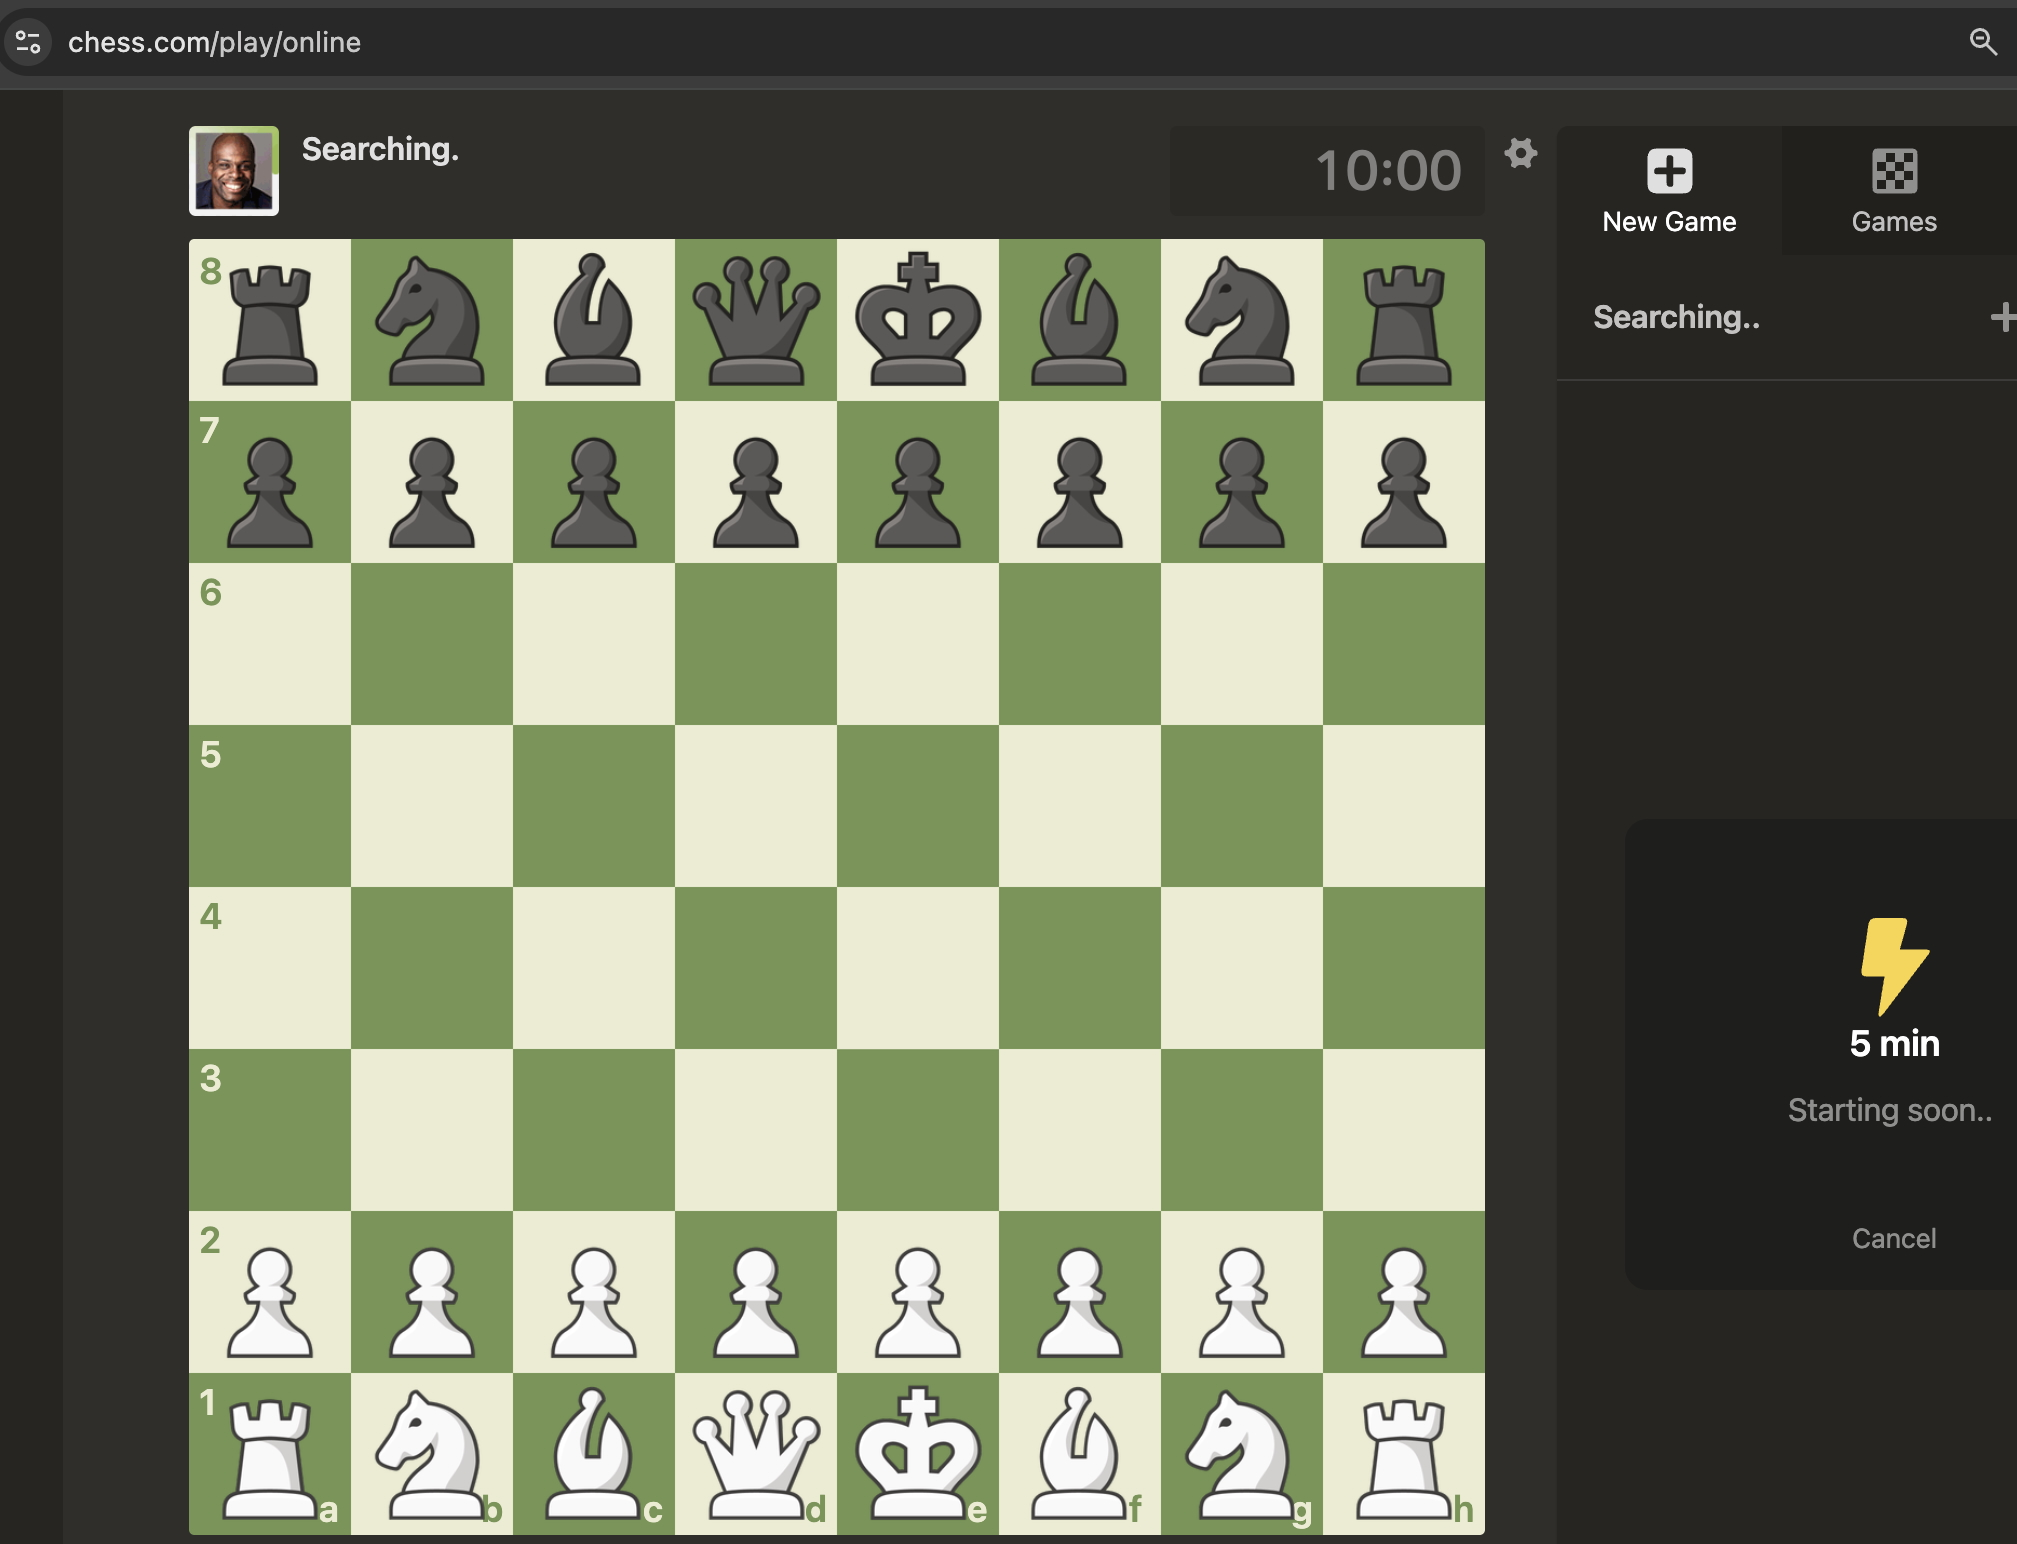
\includegraphics[height=0.8\textheight]{chesscom_search_game}\\
      {\scriptsize The live game search}
\end{frame}

\begin{frame}{What a player sees}
  \begin{columns}[T]
    \begin{column}{0.36\textwidth}
      \centering
      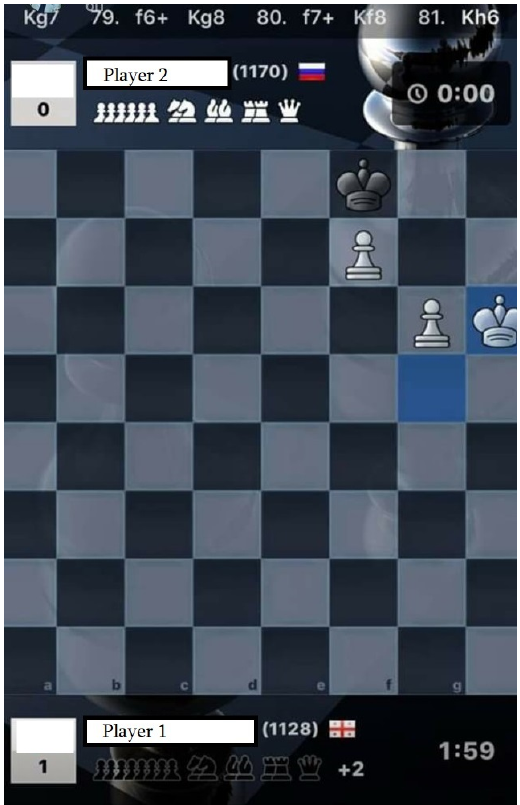
\includegraphics[height=0.62\textheight]{old_draft_fig1a_game_screenshot}\\
      {\scriptsize A live game: ratings and flags beside the names}
    \end{column}
    \begin{column}{0.36\textwidth}
      \centering
      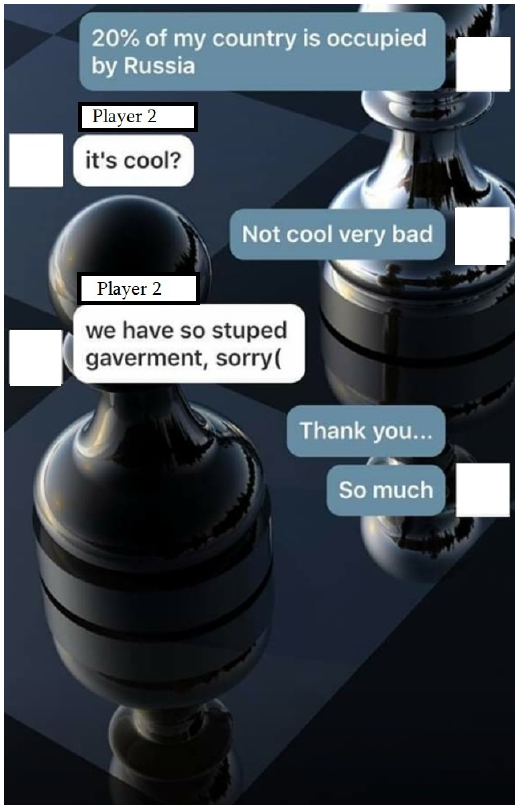
\includegraphics[height=0.62\textheight]{old_draft_fig1b_chat_screenshot}\\
      {\scriptsize In-game chat during a game}
    \end{column}
    \begin{column}{0.26\textwidth}
      \small
      \vspace{4mm}
      The opponent's flag is visible before the first move and throughout the game.\\[3mm]
      Players are paired by rating and availability; there is no way to filter opponents by country.
    \end{column}
  \end{columns}
  \src{Screenshots from the platform (May 2024 vintage); usernames and avatars removed.}
\end{frame}

\begin{frame}{Resignation: a unilateral concession}
  \begin{itemize}
    \item Either player may resign at any moment; the game ends at once as a loss for the resigner
    \item Etiquette treats resigning a clearly lost position as normal, even respectful
    \item Playing on in a lost position costs time and effort with little prospect of reward
    \item Economic theory says a contest ends when one side decides that continuing costs more than it is worth. In practice people often keep investing in a losing course of action (escalation of commitment)
    \item The platform records who conceded and when; for engine-analyzed games, also how lost the position was at that moment, i.e., the expected value of continuing/not-conceding
  \end{itemize}
\end{frame}

\begin{frame}{Research questions}
  \begin{block}{}
    Does the same player concede differently to opponents displaying the opposing country's flag once the two countries are at war?
  \end{block}
  \vspace{2mm}
  \begin{enumerate}
    \item Do players treat hostile-country opponents differently once their countries are at war?
    \item If so, which aspects of play change: whether they concede, how long they persist, the quality of their play, their choice of openings?
    \item Does any change appear wherever war breaks out, or only in some conflicts?
  \end{enumerate}
  \vspace{2mm}
  Three wars: Armenia--Azerbaijan (2020), Russia--Ukraine (2022), Israel--Palestine (2023). We measure behaviour rather than motives. Treatment is based on displayed flags, which we use as a proxy for national affiliation.
\end{frame}

\begin{frame}{Predictions around participation and performance are not obvious}
  \begin{itemize}
    \item Players may refuse to play against opponents from hostile countries, or they may want to play them more
    \item They may refuse to draw (``victory or death''), or they may be more draw-prone (``it's the governments' faults, not ours'')
    \item They may play worse due to being distracted or emotional, or they may play better due to higher perceived stakes
    \item They may resign more often to avoid the displeasure of continuing a losing game to a hostile opponent, or they may resign less often to `fight til the end' and/or disrespect their opponent
  \end{itemize}
    \vspace{2mm}
  The literature gives no clear indication of what to expect.
\end{frame}


% =====================================================================
% DATA AND DESIGN
% =====================================================================
\section{Data and design}

\begin{frame}{Three conflicts}
  \centering
  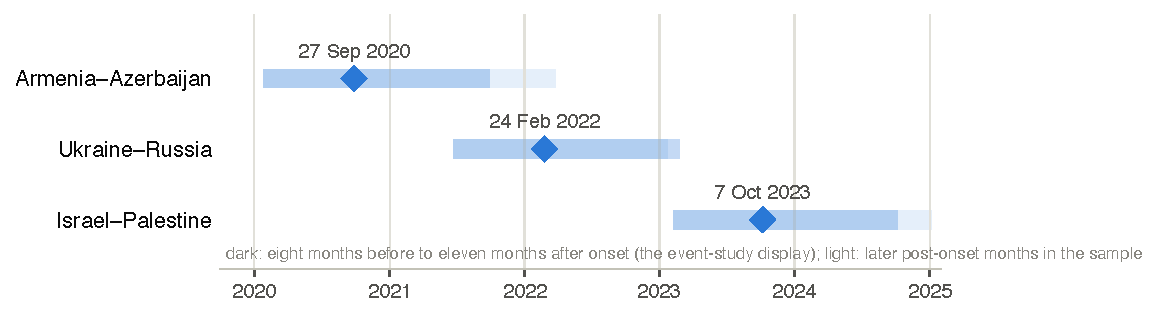
\includegraphics[width=0.86\textwidth]{timeline}
  \begin{flushleft}\small
    \begin{itemize}
      \item Treatment timing is the onset of each war, applied as an exact date
      \item Main analysis window (dark band): eight months before to eleven months after each conflict's onset; Secondary: later months in the sample (light band)
    \end{itemize}
  \end{flushleft}
  \links{\bk{bk-table1-main}{the three conflicts in numbers} \quad \fq{faq-conflicts}{why these conflicts?}}
\end{frame}

\begin{frame}[label=records]{The data: 32.4 million games by 33,687 accounts}
  \small
  \begin{itemize}
    \item Complete game records from Chess.com, a platform with more than 250 million members: who played whom and when, both ratings, every move, and how the game ended
    \item Accounts flagged to the belligerent countries were selected at random from a database assembled since 2018, on the flags they displayed before the conflict; every available game of each account is included
    \item A hostile-country game: the opponent displays the other belligerent's flag. They are 1.5\% of games; the comparison set is the same player's games against everyone else
    \item Chess players are not the public (though there are many!), and this is not a probability sample of them. The main estimand is a within-person change
  \end{itemize}
  \src{Platform scale: Chess.com country statistics article (updated 12 August 2026).}
  \links{\bk{bk-frame}{sampling frame} \quad \bk{bk-hostile}{hostile games and the comparison set} \quad \fq{faq-flags}{are flags citizenship?}}
\end{frame}

\begin{frame}[label=samples]{Two samples used in this paper}
  \small
  \begin{tabular}{@{}p{0.47\textwidth}p{0.47\textwidth}@{}}
    \textcolor{rawblue}{\textbf{Raw-record sample (primary)}} & \textcolor{engorange}{\textbf{Engine-analyzed sample}} \\
    \midrule
    32.4 million games; 33,687 accounts & 1.4 million games; 42,118 players \\[2mm]
    Every available game; no engine-based restriction & Players with more than 10 hostile-country games and more than 100 games; every hostile game kept, a random sample of other games \\[2mm]
    Outcomes: how each game ended, game length & Every move evaluated by the Stockfish engine: an objective measure of each position and each move's quality \\[2mm]
    Purpose: the behavioural result at scale & Purpose: corroborate the result under a different construction; condition on the objective position; test play quality and openings \\
  \end{tabular}
  \vspace{3mm}
  \begin{itemize}
    \item The two samples were drawn separately from the same account database; neither is a subset of the other
    \item Blue throughout for the raw records, orange for the engine-analyzed sample
  \end{itemize}
  \links{\bk{bk-eligibility}{eligibility rules} \quad \fq{faq-independent}{why two samples corroborate}}
\end{frame}

\begin{frame}[label=desc-sample]{The raw-record sample by conflict}
  \centering
  \small
  \setlength{\tabcolsep}{6pt}
  \renewcommand{\arraystretch}{1.25}
  \begin{tabular}{@{}lrrrrr@{}}
    \toprule
    & \multicolumn{2}{c}{Accounts} & \multicolumn{2}{c}{Player-game observations} & Games per \\
    \cmidrule(lr){2-3}\cmidrule(lr){4-5}
    Conflict & Number & Share & Number & Share & account (mean) \\
    \midrule
    Armenia--Azerbaijan & 9,005 & 26.7\% & 13,363,927 & 37.2\% & 1,484 \\
    Ukraine--Russia & 14,658 & 43.5\% & 15,668,875 & 43.6\% & 1,069 \\
    Israel--Palestine & 10,024 & 29.8\% & 6,904,679 & 19.2\% & 689 \\
    \midrule
    Pooled & 33,687 & 100\% & 35,937,481 & 100\% & 1,067 \\
    \bottomrule
  \end{tabular}
  \vspace{3mm}
  \begin{flushleft}\small
    \begin{itemize}
      \item A player-game observation is one sampled player's side of one game. Ukraine--Russia contributes the most accounts and the most observations
      \item Games per account is observations divided by accounts over the whole sample window. It is a mean: activity differs greatly across players, which is why we report estimates weighted per game and per player
    \end{itemize}
  \end{flushleft}
  \links{\bk{bk-table1-main}{Table 1 with physical games} \quad \bk{bk-table1}{counting conventions}}
\end{frame}

\begin{frame}[label=desc-contact]{How often players meet the other side}
  \centering
  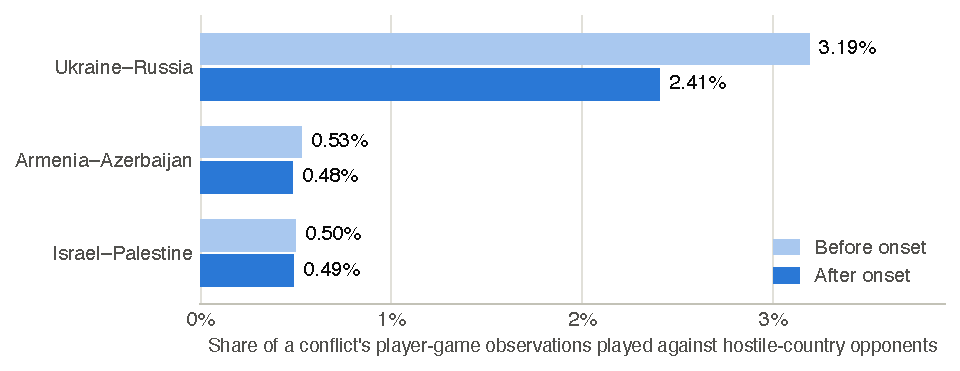
\includegraphics[width=0.72\textwidth]{hostile_share_prepost}
  \begin{flushleft}\small
    \begin{itemize}
      \item Hostile-country games are rare. Before onset they were about 2\% of player-game observations (1.98\% pooled); 18,852 accounts played at least one. The same players' other games are the comparison set
      \item The share is lower after onset, most clearly in Ukraine--Russia: many Ukrainian players stopped playing in the first weeks of the war, and Russia blocked the platform on 23 April 2022. Whether players also avoided these games is taken up under Limitations
    \end{itemize}
  \end{flushleft}
  \links{\bk{bk-contact}{Ukraine--Russia month by month} \quad \bk{bk-hostile}{hostile games and the comparison set} \quad \hyperlink{flags}{\textcolor{linkblue}{\scriptsize\textsf{limitations}}}}
\end{frame}

\begin{frame}[label=desc-balance]{Hostile-country games and other games before the war}
  \centering
  \small
  \setlength{\tabcolsep}{10pt}
  \renewcommand{\arraystretch}{1.3}
  \begin{tabular}{@{}lrr@{}}
    \toprule
    Before onset, raw-record sample, three conflicts pooled & \shortstack[r]{Hostile-country\\games} & \shortstack[r]{All other\\games} \\
    \midrule
    Player-game observations & 0.41 million & 20.33 million \\
    Accounts with at least one such game & 18,852 & 32,584 \\
    The player resigned & 21.46\% & 20.34\% \\
    The game ended in a resignation by either player & 43.26\% & 41.43\% \\
    Game length (moves) & 35.9 & 35.0 \\
    \bottomrule
  \end{tabular}
  \vspace{3mm}
  \begin{flushleft}\small
    \begin{itemize}
      \item Before the war, hostile-country games already differed a little from other games
      \item The design does not need the two kinds of game to look alike. It needs the gap between them to have stayed the same had the war not begun; the estimate is the change in that gap
    \end{itemize}
  \end{flushleft}
  \links{\bk{bk-hostile}{the comparison set}}
\end{frame}

\begin{frame}[label=comparison]{Estimation: the same player, two kinds of opponent, before and after}
  \centering
  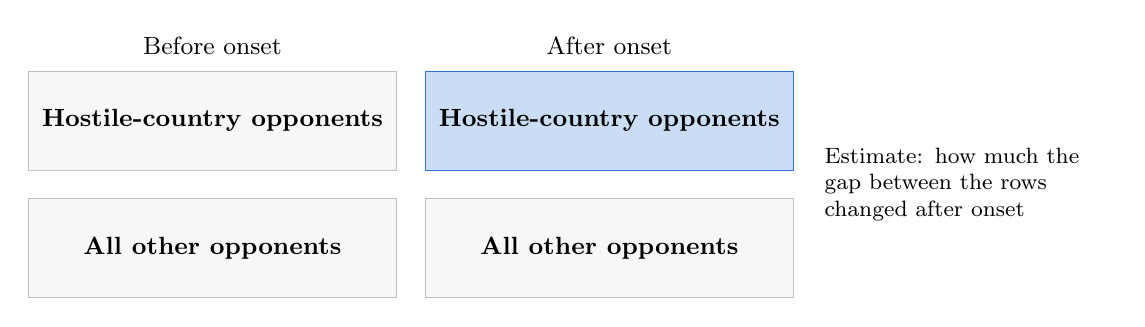
\begin{tikzpicture}[x=0.9mm,y=0.9mm,font=\small]
    \draw[fill=black!3,draw=black!25] (0,0) rectangle (52,14);
    \draw[fill=black!3,draw=black!25] (56,0) rectangle (108,14);
    \draw[fill=black!3,draw=black!25] (0,18) rectangle (52,32);
    \draw[fill=rawblue!25,draw=rawblue] (56,18) rectangle (108,32);
    \node at (26,25) {\textbf{Hostile-country opponents}};
    \node at (26,7) {\textbf{All other opponents}};
    \node at (82,25) {\textbf{Hostile-country opponents}};
    \node at (82,7) {\textbf{All other opponents}};
    \node[anchor=south] at (26,33) {Before onset};
    \node[anchor=south] at (82,33) {After onset};
    \node[anchor=west,font=\footnotesize,text width=36mm] at (111,16) {Estimate: how much the gap between the rows changed after onset};
  \end{tikzpicture}
  \vspace{2mm}
  \begin{flushleft}\small
    \begin{itemize}
      \item Within each player and each calendar month of each conflict: player fixed effects absorb everything stable about a player; conflict-by-month effects absorb activity waves and platform-wide shocks; both ratings controlled; standard errors clustered by player
      \item The assumption: without the onset, the gap between a player's hostile-country games and their other games would have followed a similar path
    \end{itemize}
  \end{flushleft}
  \links{\bk{bk-fe}{what the fixed effects absorb} \quad \bk{bk-ident}{identification in words} \quad \fq{faq-lpm}{why a linear model?}}
\end{frame}

\begin{frame}[label=equation]{Estimation: the specification}
  For outcome $Y$ of focal player $i$ in game $g$, in calendar month $m$ of conflict sample $s$:
  \vspace{2mm}
  \begin{equation*}
    Y_{igsm} = \beta\,(\mathrm{Hostile}_{ig}\times\mathrm{Post}_{g}) + \gamma\,\mathrm{Hostile}_{ig}
    + \theta\,\mathrm{Rating}_{im} + \varphi\,\mathrm{OppRating}_{g} + \alpha_i + \lambda_{sm} + \varepsilon_{igsm}
  \end{equation*}
  \vspace{1mm}
  \small
  \begin{itemize}
    \item $\beta$ is the estimand: the change in the hostile-versus-other gap at onset, within player and within calendar month
    \item $\alpha_i$: player fixed effects. $\lambda_{sm}$: conflict-sample-by-calendar-month effects, which absorb the post-onset main effect and any conflict-specific calendar shock. $\mathrm{Hostile}_{ig}$: the opponent displays the other belligerent's flag; $\mathrm{Post}_g$: the game is played after onset
    \item Linear probability model; effects in percentage points; standard errors clustered by focal player
    \item Two weightings: each game equally (the per-game estimate) and each player equally (the per-player estimate)
  \end{itemize}
  \links{\fq{faq-lpm}{why a linear probability model?} \quad \bk{bk-robust}{robustness dimensions} \quad \bk{bk-fe}{what the fixed effects absorb}}
\end{frame}

\begin{frame}[label=before]{Before onset: no pre-trend}
  \centering
  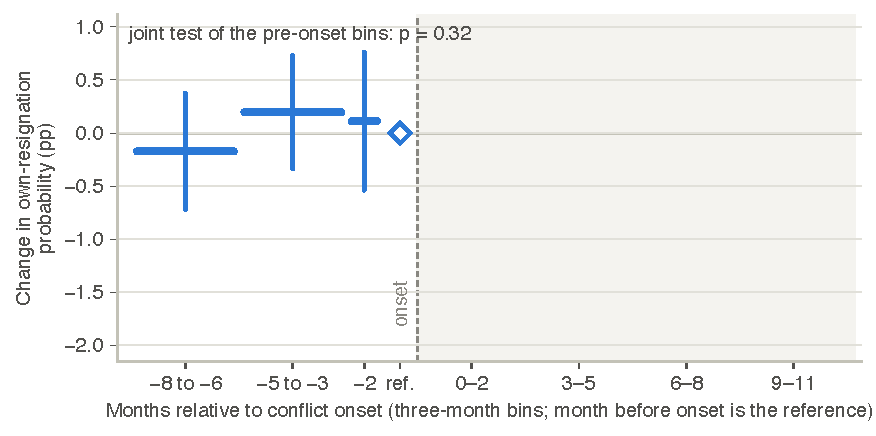
\includegraphics[width=0.66\textwidth]{event_pre}
  \begin{flushleft}\small
    \begin{itemize}
      \item Each bar: the change in the gap in that three-month bin relative to the month before onset (``ref.''); zero means no change; the vertical lines are 95\% confidence intervals
      \item The three pre-onset bins are jointly indistinguishable from zero ($p = .32$)
    \end{itemize}
  \end{flushleft}
  \links{\bk{bk-monthly}{monthly version} \quad \bk{bk-pretrends}{per-conflict tests} \quad \fq{faq-pretrends}{why should these be zero?}}
\end{frame}

\begin{frame}[label=after]{After onset: negative in every bin}
  \centering
  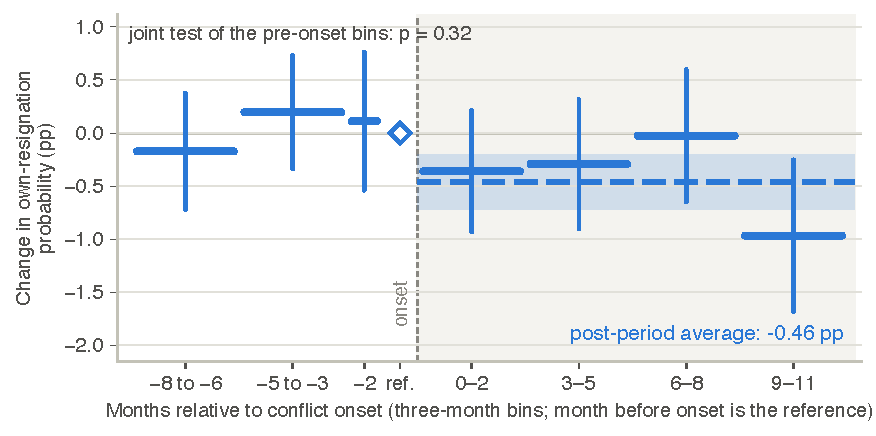
\includegraphics[width=0.66\textwidth]{event_post}
  \begin{flushleft}\small
    \begin{itemize}
      \item Every post-onset bin is negative; the dashed line is the full post-period estimate ($-0.46$ pp, each game equally); months 6--8 sit near zero and the largest decline is in months 9--11
      \item The display stops at month 11, where Ukraine--Russia, the largest conflict, leaves the window; later bins rest on fewer conflicts
    \end{itemize}
  \end{flushleft}
  \links{\bk{bk-fullwindow}{bins to month 17}}
\end{frame}

% =====================================================================
% HEADLINE (moved after the event study at David's request, 2026-10-03)
% =====================================================================
\section{The headline}

\begin{frame}[label=headline]{Players conceded less often to hostile-country opponents after war began}
  \centering
  \only<1>{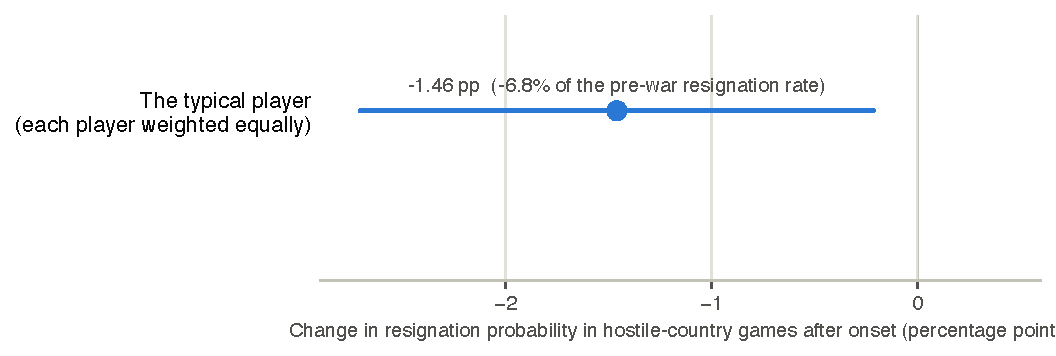
\includegraphics[width=0.72\textwidth]{headline_step1}}%
  \only<2>{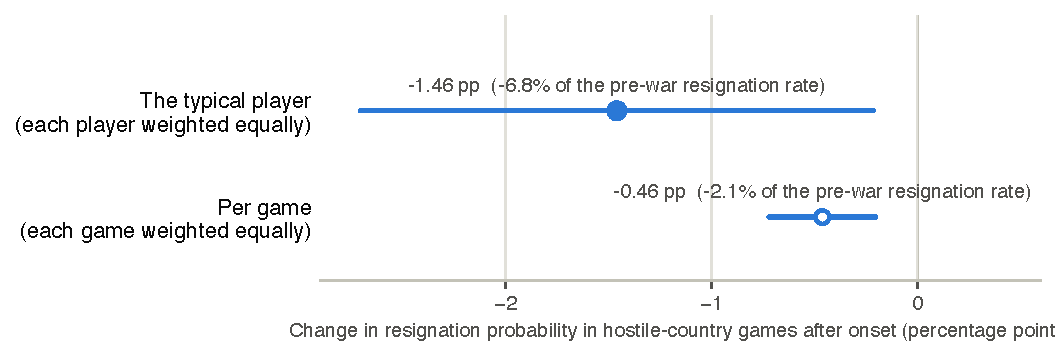
\includegraphics[width=0.72\textwidth]{headline_step2}}
  \begin{flushleft}\small
    \begin{itemize}
      \item Same player, hostile-country games versus all their other games, after versus before onset; each player weighted equally: $-1.46$ percentage points, 6.8\% of the pre-war resignation rate in hostile-country games (SE 0.64 pp, $p = .022$). Roughly 3 fewer resignations in every 100 games the player loses (next slide)
      \item<2-> Each game weighted equally, an average dominated by the most active players: $-0.46$ pp, 2.1\% of the pre-war rate (SE 0.13 pp, $p = .0005$)
      \item<2-> Not in every war: Armenia--Azerbaijan shows no detectable change (coming up)
    \end{itemize}
  \end{flushleft}
  \links{\fq{faq-magnitude}{what does this mean concretely?}}
\end{frame}

\begin{frame}[label=scale]{How big is that? Measured against the games a player loses}
  \centering
  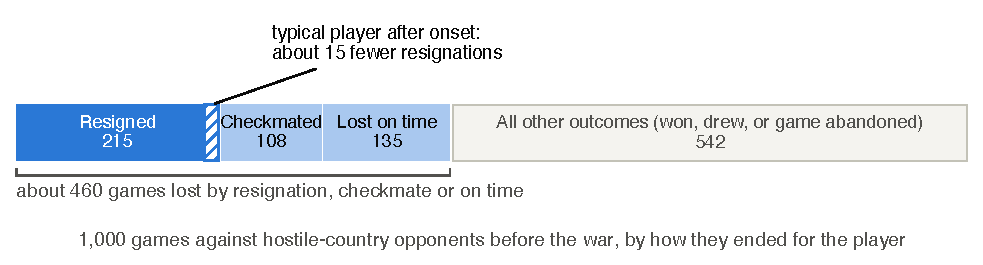
\includegraphics[width=0.78\textwidth]{scale_lost_games}
  \begin{flushleft}\small
    \begin{itemize}
      \item A player almost always only resigns games they are losing. Before the war players lost about 460 of every 1,000 hostile-country games by resignation, checkmate or on time; about 215 of those were resignations, about 47\% of lost games
      \item The typical player after onset resigned about 15 fewer of those games: about 200 of the 460 lost games ended with a resignation instead of 215. That is about 44\% of lost games instead of 47\%, or roughly 3 fewer resignations in every 100 lost games
      \item The losses did not become rarer; they ended differently, in checkmate or on the clock (coming up)
    \end{itemize}
  \end{flushleft}
  \links{\fq{faq-magnitude}{the arithmetic, step by step} \quad \hyperlink{endings}{\textcolor{linkblue}{\scriptsize\textsf{where the concessions went}}}}
\end{frame}

\begin{frame}[label=whoseaverage]{Per-player vs per-game estimates}
  \begin{columns}[T]
    \begin{column}{0.56\textwidth}
      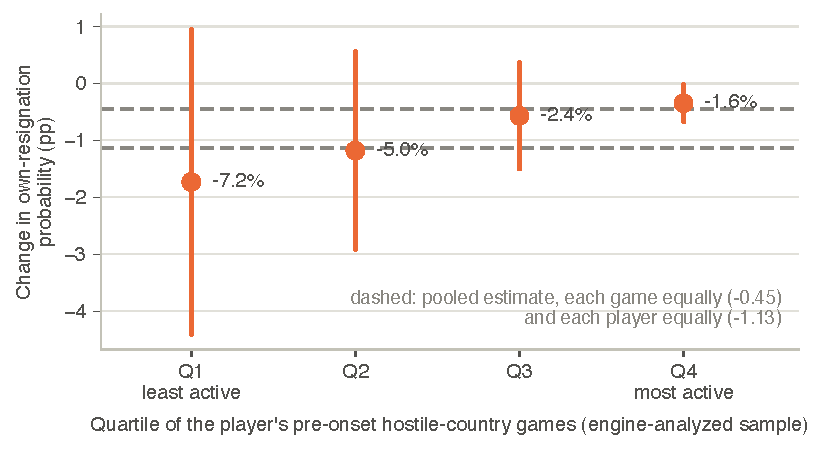
\includegraphics[width=\textwidth]{activity_gradient}
    \end{column}
    \begin{column}{0.44\textwidth}
      \small
      \begin{itemize}
        \item The per-game estimate weights each player by games played, so a threefold gap means the most active players changed least
        \item Players grouped by how many hostile-country games they played before the war: estimates shrink from the least to the most active quarter and span the two averages (differences between quarters are imprecise)
        \item Occasional participants changed most: a comparison across players (less active players respond more), not an effect that fades within a player with repeated contact
      \end{itemize}
    \end{column}
  \end{columns}
  \links{\bk{bk-activity}{quartile table} \quad \bk{anyone}{is anyone driving it?} \quad \fq{faq-weighting}{why equal weighting triples the estimate}}
\end{frame}



% =====================================================================
% RESULTS
% =====================================================================
\section{Results}

\begin{frame}[label=byconflict]{By conflict}
  \centering
  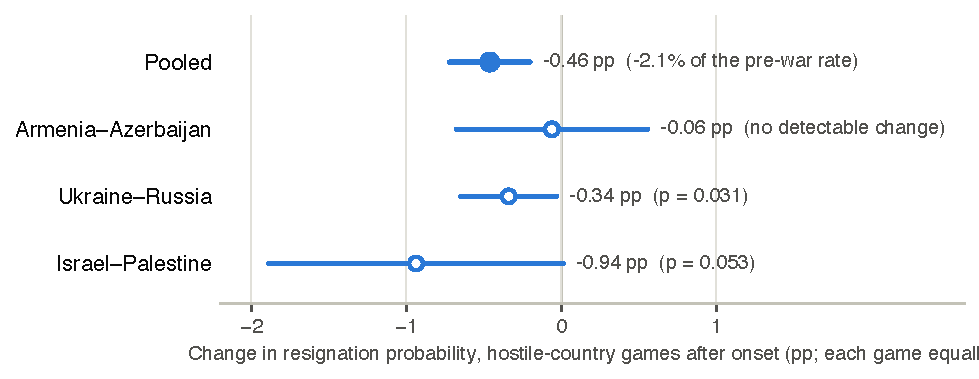
\includegraphics[width=0.8\textwidth]{forest_raw}
  \begin{flushleft}\small
    \begin{itemize}
      \item Ukraine--Russia and Israel--Palestine decline; Armenia--Azerbaijan shows no detectable change. Dropping any one conflict leaves the pooled estimate negative
    \end{itemize}
  \end{flushleft}
  \links{\bk{bk-forest-full}{both samples by conflict} \quad \bk{bk-loo}{leave-one-conflict-out}}
\end{frame}

\begin{frame}[label=boundary]{Armenia--Azerbaijan}
  \begin{itemize}
    \item No detectable change in resignation in either sample: $-0.06$ pp ($p = .85$) in the raw records, $+0.12$ pp ($p = .78$) in the engine-analyzed sample
    \item Possible explanation (not testable in our data): active hostilities ended with a ceasefire about six weeks after onset, so most of the post-onset window lies after the fighting had ceased
    \item This conflict moves on a different margin, departures from habitual openings (later)
  \end{itemize}
  \links{\bk{bk-aalength}{game length in this dyad} \quad \fq{faq-aa}{why is it null?}}
\end{frame}

\begin{frame}[label=corroboration]{Consistency of results across samples}
  \centering
  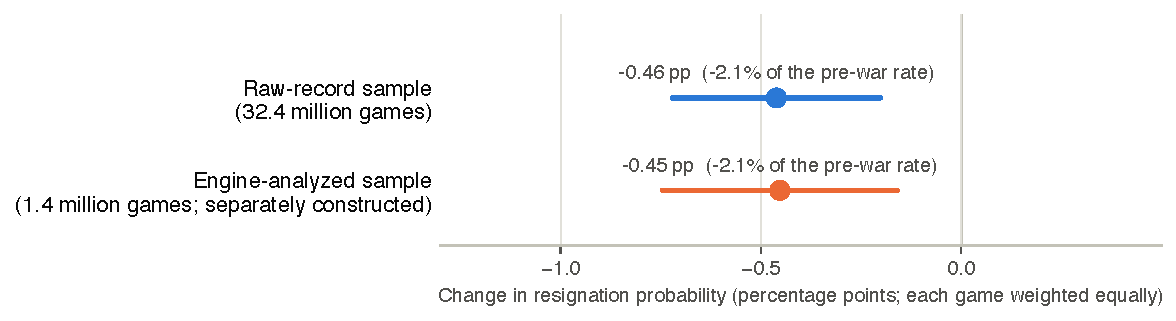
\includegraphics[width=0.8\textwidth]{corroboration}
  \begin{flushleft}\small
    \begin{itemize}
      \item Different eligibility rules, different sampling of comparison games, a different data path; the per-game estimate reproduces almost exactly, and so do the per-conflict pattern and the weighting contrast (each player equally: $-1.13$ pp, about 2.5 times the per-game estimate)
    \end{itemize}
  \end{flushleft}
  \links{\bk{bk-forest-full}{by conflict, both samples} \quad \fq{faq-independent}{why this counts as corroboration}}
\end{frame}

\begin{frame}[label=endings]{Where the missing concessions went: checkmate, or the clock}
  \centering
  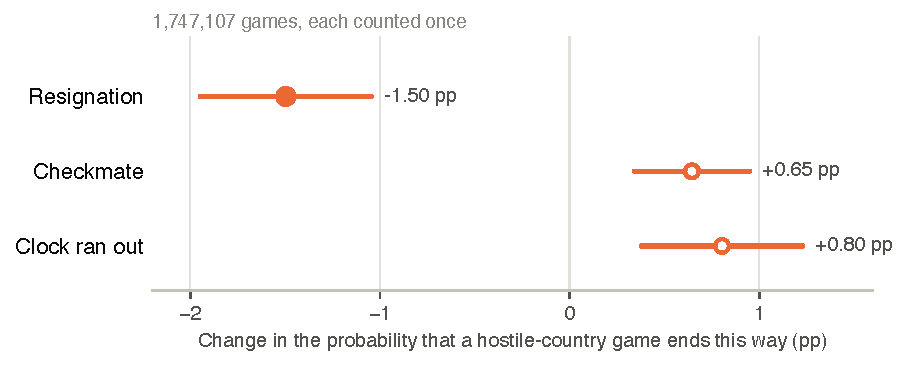
\includegraphics[width=0.74\textwidth]{endings}
  \begin{flushleft}\small
    \begin{itemize}
      \item Each game counted once: resignation endings fell by 1.50 pp; checkmates rose by 0.65 and losses on time by 0.80, together $+1.45$ pp. Games that would have ended in concession ran on to checkmate or until a clock ran out
      \item Whether games were decisive, and every kind of draw, did not change; games became slightly longer ($+0.45$ moves) as a result
    \end{itemize}
  \end{flushleft}
  \links{\bk{bk-composition-full}{draws and game length} \quad \bk{bk-gamelevel}{game-level estimation}}
\end{frame}

\begin{frame}[label=lostdef]{Measuring continuation after a position is lost}
  \begin{columns}[T]
    \begin{column}{0.55\textwidth}
      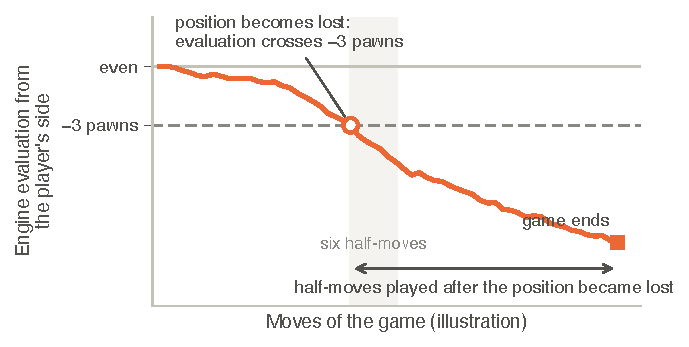
\includegraphics[width=\textwidth]{eval_schematic_v3}
    \end{column}
    \begin{column}{0.45\textwidth}
      \small
      \vspace{2mm}
      \begin{itemize}
        \item The engine evaluates every position. A position counts as lost when the evaluation first falls to three pawns or worse against the player, which at these levels is almost always decisive
        \item The risk set is every game in which that happened: 1,115,113 player-game observations from 35,925 players. Membership never depends on how the game ended
        \item Two measures of continuing: the half-moves played after the position became lost, and whether the player went on for more than six half-moves
      \end{itemize}
    \end{column}
  \end{columns}
  \links{\fq{faq-glossary}{half-moves, pawns, centipawns}}
\end{frame}

\begin{frame}[label=persistence]{Players fought on longer in positions that were already lost}
  \centering
  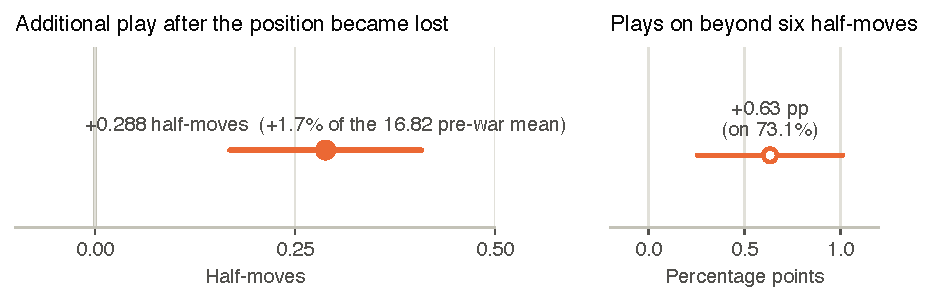
\includegraphics[width=0.84\textwidth]{persistence_v3}
  \begin{flushleft}\small
    \begin{itemize}
      \item Against hostile-country opponents after onset, players played $+0.288$ more half-moves per lost game (SE 0.061, $p < .0001$), a 1.7\% increase on the pre-war mean, and were more likely to continue beyond six half-moves ($+0.63$ pp on 73.05\%, $p = .0011$)
      \item The cost falls on the persister: time and effort in positions offering essentially no prospect of reward
    \end{itemize}
  \end{flushleft}
  \links{\bk{bk-persistence-full}{all persistence measures} \quad \bk{bk-persistconflict}{by conflict}}
\end{frame}

\begin{frame}[label=checks]{Robustness: the same games became lost, and players did not move their threshold}
  \centering
  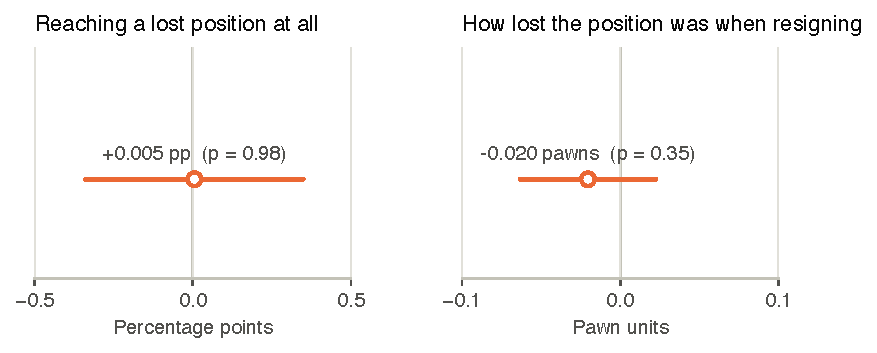
\includegraphics[width=0.72\textwidth]{guards_v3}
  \begin{flushleft}\small
    \begin{itemize}
      \item The probability that a game ever reached a lost position did not change, so the extra persistence is not more games entering the risk set
      \item The engine's evaluation at the moment a player resigned did not change, so players did not simply relocate the point at which they give up
    \end{itemize}
  \end{flushleft}
  \links{\bk{bk-rating}{by rating} \quad \fq{faq-worseplay}{could it be worse play?}}
\end{frame}

\begin{frame}[label=quality]{Move quality: do players play worse?}
  \centering
  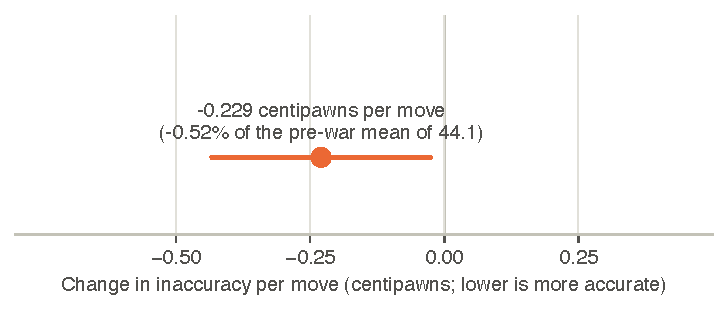
\includegraphics[width=0.8\textwidth]{quality_main}
  \begin{flushleft}\small
    \begin{itemize}
      \item The engine scores every move against its best move; the per-move error fell slightly in hostile-country games after onset (SE 0.104, $p = .027$), and performance relative to what the ratings predicted did not change ($p = .83$)
      \item Whatever kept players fighting in lost positions, it was not accompanied by deteriorating play
    \end{itemize}
  \end{flushleft}
  \links{\bk{bk-quality-full}{three quality measures} \quad \bk{bk-secondary}{secondary outcomes}}
\end{frame}

\begin{frame}[label=openings]{A different margin: departures from habitual openings}
  \centering
  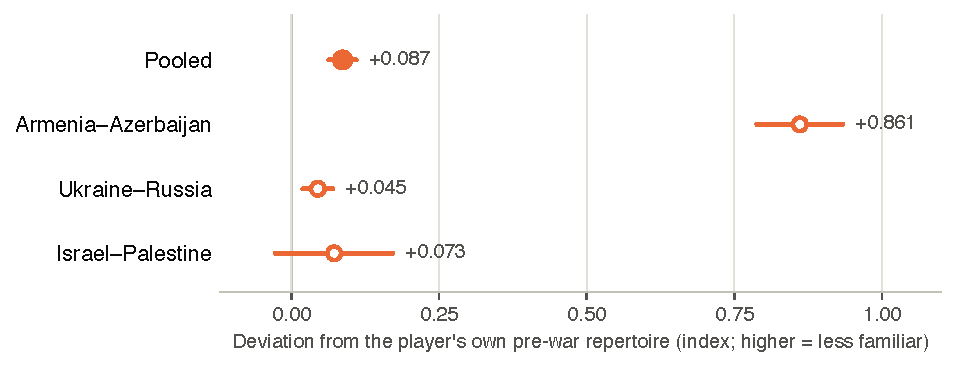
\includegraphics[width=0.62\textwidth]{openings_main}
  \begin{flushleft}\footnotesize
    \begin{itemize}
      \item Chess players typically stick to a familiar set of initial moves, or ``openings'', that make up an individual's ``opening repertoire''
      \item Each opening is scored against the player's own pre-war repertoire (minus the log of how often they had used it; $+0.1$ is an opening used about 10\% less often before the war). Hostile-country games: $+0.087$ after onset, 2.2\% of the pre-war mean ($p < .0001$)
      \item Armenia--Azerbaijan, which shows no resignation change, shows the biggest openings effect: players departed from their usual repertoire. If anything, the share of aggressive openings fell, but the estimate is noisy, and the share of safe openings did not rise
    \end{itemize}
  \end{flushleft}
  \links{\bk{bk-openings-full}{by colour; without Armenia--Azerbaijan} \quad \bk{bk-openings}{the index}}
\end{frame}

\begin{frame}[label=sensitivity]{Sensitivity to analysis choices: specification curve}
  \centering
  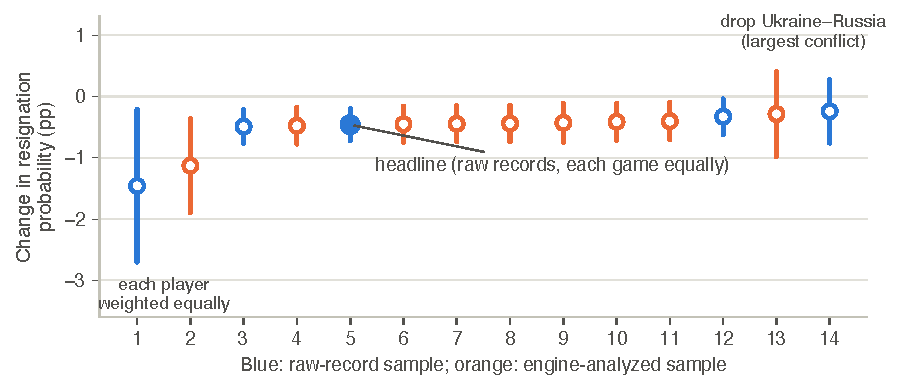
\includegraphics[width=0.84\textwidth]{spec_curve_simple}
  \begin{flushleft}\small
    \begin{itemize}
      \item Fourteen already-reported specifications: sample, weighting, conflicts included, fixed effects, comparison group, duplicate records. The two widest intervals drop the largest conflict; the two largest declines weight each player equally
    \end{itemize}
  \end{flushleft}
  \links{\bk{bk-speccurve-full}{with the choice matrix} \quad \bk{bk-robust}{dimensions tested}}
\end{frame}

\begin{frame}[label=flags]{Limitations}
  \small
  \begin{itemize}
    \item A displayed flag is not necessarily citizenship. Each account is classified by one recorded flag, taken before the war for focal players, so the sample cannot respond to the war. Accounts that later changed flag are not dropped; they are few (94.0\% of accounts in the full database showed the same flag seven years on). A game against an opponent who had changed flag is an untreated game counted as treated, which pulls the estimate toward zero. The largest movement, an inflow into the Palestinian flag, matters for Israel--Palestine only
    \item Players cannot filter opponents by country; pairing is by rating and availability. Who is online at a given moment is not fixed, and the month effects absorb only changes common to a conflict's players
    \item Games aborted before the first move are not stored, so a player who leaves on seeing the flag is invisible; abandonment inside stored games did not change ($+0.08$ pp, $p = .16$)
    \item Contact with the other side fell after onset, most in Ukraine--Russia. The fall follows Russia's block of the platform on 23 April 2022, not the onset of the war, which points to the supply of opponents; avoidance by some players cannot be ruled out
  \end{itemize}
  \links{\bk{bk-contact}{contact by month} \quad \bk{threats}{threats table} \quad \bk{bk-flags}{flag audit} \quad \fq{faq-quit}{quit on seeing the flag?}}
\end{frame}

% =====================================================================
% INTERPRETATION AND CLOSE
% =====================================================================
\section{Interpretation}

\begin{frame}{What does it mean to keep playing a lost position?}
  \small
  Several interpretations are consistent with the pattern of results; the data record behaviour, not motive, and we do not adjudicate.
  \begin{enumerate}
    \item \textbf{Withholding the acknowledgment of victory.} Resignation hands the opponent an acknowledged win. Fits the shift of endings to checkmate and time, the unchanged evaluation at resignation, and no decline in quality
    \item \textbf{Higher stakes under rivalry.} Losing to this opponent may simply have mattered more; an escalation-of-commitment pattern
    \item \textbf{Wartime suspension of courtesies.} Resignation is etiquette, a concession granted as much as a defeat accepted
  \end{enumerate}
  \begin{itemize}
    \item What we can say: the behaviour had a real price, additional play in positions already objectively lost, which separates it from cheap talk
    \item What is not certain: identity salience and nationalism were not measured; chess players are a selected population; flags are not necessarily citizenship; the Armenia--Azerbaijan hypothesis is untested
  \end{itemize}
\end{frame}

\begin{frame}{Possible implications for business interactions}
  \begin{itemize}
    \item The transferable object is the decision to ``concede'', or accept an end. Transferable applications would need to measure the route to an ending, the effort spent reaching it, and the task quality separately
    \item Candidate settings where all three are plausibly recorded: commercial disputes and settlements; loan covenant waivers; marketplace and freelance disputes (refund, chargeback, abandonment)
    \item Candidate outcomes: voluntary resolution versus formal decision or expiry; time to resolution and both parties' costs; independently assessed quality of the underlying work
    \item Plus, more broadly, online digital (strategic) interactions between individuals
  \end{itemize}
  \links{\fq{faq-structural}{is there a model behind this?}}
\end{frame}

\begin{frame}[label=nextsteps]{Next steps}
  \small
  \begin{itemize}
    \item \textbf{A preregistered out-of-sample replication: the Iran war} (onset February 2026). The specification was frozen before anyone examined Iranian data; the September 2024 account re-scrape predates the onset, so focal players can be sampled on pre-conflict flags. Plan: timestamp a pre-analysis plan now; run once a longer post-onset window exists
    \item Does the effect fade with repeated contact? A within-player test by the order of a player's post-onset hostile-country games (exploratory run done; raw-record replication pending)
    \item Rematches: after a game, did the same two players play again straight away? Both are already online and paired, so the supply of opponents is held fixed: a direct test of whether players avoid the other side (planned, on the full records)
    \item Moderators, none tested here: conflict duration, intensity, diaspora composition, platform exposure
    \item A structural interpretation of continuation decisions in lost positions is companion work in progress
  \end{itemize}
  \links{\bk{bk-iran}{Iran feasibility}}
\end{frame}

\begin{frame}{Conclusion}
  \small
  \begin{block}{}
    War changes everyday behaviour: after onset, individuals became reluctant to concede to the other side, in contests far removed from the fighting
  \end{block}
  \vspace{2mm}
  \begin{itemize}
    \item About 7\% of the pre-conflict resignation rate for the typical player, about 2\% per game; the per-game estimate reproduces almost exactly in a separately built sample
    \item Fewer concessions became checkmates and losses on time; players persisted in positions already objectively lost, without playing worse
    \item Not in every war: no change in Armenia--Azerbaijan, which moved instead on the openings margin
  \end{itemize}
\end{frame}

\appendix
\section{Backup}

\begin{frame}[label=backup-index]{Backup slides (1 of 2): data, design, specification}
  \footnotesize
  \begin{columns}[T]
    \begin{column}{0.5\textwidth}
      \textbf{Sampling and data}
      \begin{itemize}
        \item \hyperlink{bk-table1-main}{The three conflicts (Table 1)}
        \item \hyperlink{bk-hostile}{Hostile games and the comparison set}
        \item \hyperlink{bk-eligibility}{Eligibility rules}
        \item \hyperlink{bk-frame}{Sampling frame}
        \item \hyperlink{bk-flags}{Flag-stability audit}
        \item \hyperlink{bk-flagmeaning}{What a flag is and is not}
        \item \hyperlink{bk-table1}{Counting conventions}
        \item \hyperlink{bk-2014}{The 2014 robustness sample}
      \end{itemize}
    \end{column}
    \begin{column}{0.5\textwidth}
      \textbf{Design and specification}
      \begin{itemize}
        \item \hyperlink{bk-ident}{Identification in words; platform facts}
        \item \hyperlink{bk-fe}{What the fixed effects absorb}
        \item \hyperlink{threats}{Threats to identification}
        \item \hyperlink{bk-robust}{Robustness dimensions tested}
        \item \hyperlink{bk-gamelevel}{Game-level estimation}
        \item \hyperlink{bk-lit1}{Literature: conflict and parochialism}
        \item \hyperlink{bk-lit2}{Literature: markets, institutions, expression}
      \end{itemize}
    \end{column}
  \end{columns}
  \links{\hyperlink{backup-index2}{\textcolor{linkblue}{\scriptsize\textsf{backup (2 of 2)}}} \quad \hyperlink{faq-index}{\textcolor{linkblue}{\scriptsize\textsf{FAQ index}}}}
\end{frame}

\begin{frame}[label=backup-index2]{Backup slides (2 of 2): results in full, dynamics, heterogeneity}
  \footnotesize
  \begin{columns}[T]
    \begin{column}{0.5\textwidth}
      \textbf{Results in full}
      \begin{itemize}
        \item \hyperlink{bk-forest-full}{Per-conflict estimates, both samples}
        \item \hyperlink{bk-loo}{Leave-one-conflict-out}
        \item \hyperlink{bk-composition-full}{All endings and draws}
        \item \hyperlink{bk-persistence-full}{All persistence measures}
        \item \hyperlink{bk-persistconflict}{Persistence by conflict}
        \item \hyperlink{bk-quality-full}{Three quality measures}
        \item \hyperlink{bk-secondary}{Quality and secondary outcomes}
        \item \hyperlink{bk-openings-full}{Openings by colour}
        \item \hyperlink{bk-openings}{The deviation index}
        \item \hyperlink{bk-aalength}{Game length in Armenia--Azerbaijan}
        \item \hyperlink{bk-speccurve-full}{Specification curve with matrix}
      \end{itemize}
    \end{column}
    \begin{column}{0.5\textwidth}
      \textbf{Dynamics}
      \begin{itemize}
        \item \hyperlink{bk-monthly}{Monthly event studies}
        \item \hyperlink{bk-fullwindow}{Bins to month 17}
        \item \hyperlink{bk-pretrends}{Per-conflict pre-trend tests}
        \item \hyperlink{bk-contact}{Ukraine--Russia: contact by month}
      \end{itemize}
      \textbf{Heterogeneity and other}
      \begin{itemize}
        \item \hyperlink{anyone}{Is anyone driving it?}
        \item \hyperlink{bk-dispersion}{Dispersion of player-level effects}
        \item \hyperlink{bk-rating}{Rating quartiles}
        \item \hyperlink{bk-activity}{Activity quartiles}
        \item \hyperlink{bk-ethics}{Ethics and data governance}
        \item \hyperlink{bk-iran}{Iran feasibility}
      \end{itemize}
    \end{column}
  \end{columns}
  \links{\hyperlink{backup-index}{\textcolor{linkblue}{\scriptsize\textsf{backup (1 of 2)}}} \quad \hyperlink{faq-index}{\textcolor{linkblue}{\scriptsize\textsf{FAQ index}}}}
\end{frame}

\begin{frame}[label=bk-table1-main]{Backup: the three conflicts and the analysis samples}
  \centering
  \footnotesize
  \setlength{\tabcolsep}{4pt}
  \begin{tabular}{@{}llrrrr@{}}
    \toprule
    Conflict & Onset & Accounts & Physical games & Player-game obs. & \shortstack[r]{Pre-onset resignation\\rate, hostile games} \\
    \midrule
    Armenia--Azerbaijan & 27 Sep 2020 & 9,005 & 11,561,545 & 13,363,927 & 18.68\% \\
    Russia--Ukraine & 24 Feb 2022 & 14,658 & 14,929,869 & 15,668,875 & 21.82\% \\
    Israel--Palestine & 7 Oct 2023 & 10,024 & 5,955,018 & 6,904,679 & 19.17\% \\
    \midrule
    Pooled & & 33,687 & 32,394,475 & 35,937,481 & 21.46\% \\
    \bottomrule
  \end{tabular}
  \vspace{2mm}
  \begin{flushleft}\footnotesize
    \begin{itemize}
      \item Raw-record sample, dyad-restricted: a focal player enters only through the sample of their own conflict
      \item Player-game observations count each game from the sampled player's side; a game between two sampled players appears once per perspective
      \item A game whose two players belong to different conflict samples is counted in both per-conflict rows but once in the pooled row, so the physical-game column sums above the pooled total
      \item The Ukraine--Russia 2014 sample (1,173 accounts; 1,187,263 physical games; 1,276,315 observations) sits outside the pooled analysis and serves for robustness
    \end{itemize}
  \end{flushleft}
  \links{\bk{bk-table1}{counting conventions} \quad \bk{bk-2014}{the 2014 sample} \quad \hyperlink{records}{\textcolor{linkblue}{\scriptsize\textsf{back: the records}}}}
\end{frame}

\begin{frame}[label=bk-hostile]{Backup: hostile-country games and the comparison set}
  \begin{itemize}
    \item Hostile-country game: the opponent's displayed country is the other belligerent of the player's own conflict
    \item 476,920 hostile physical games, 1.5\% of the 32,394,475: the treated set is small by design; the comparison set is meant to dwarf it
    \item Comparison set: the same player's games against everyone else. Of these, 90.9\% are against third-country opponents, 6.1\% same-country, 3.0\% opponents from countries involved in one of the other conflicts (classified with a frozen list)
    \item Unit of observation: one focal player's perspective on one game (a player-game observation)
    \item Precision comes from the within-player contrast between the hostile games and the far larger comparison set
    \item Throughout: ``hostile-country opponent'' means this displayed-country definition; a displayed flag is never citizenship
  \end{itemize}
  \links{\bk{bk-robust}{robustness dimensions} \quad \fq{faq-flags}{are flags citizenship?}}
\end{frame}

\begin{frame}[label=bk-ident]{Backup: identification in words, and the platform facts}
  \small
  \begin{block}{}
    We compare the same player's behaviour against hostile-country opponents with that player's behaviour against everyone else, before versus after their countries' war began. Identification requires that, absent onset, that gap would have evolved in parallel.
  \end{block}
  \vspace{2mm}
  \textbf{Institutional facts}
  \begin{itemize}
    \item Players cannot block or filter opponents by country; the platform offers no such option
    \item Matchmaking: ``When you choose your time control, we try to find you an opponent who is closest to your current rating.''
    \item Onset timing is not driven by any player; pairing, conditional on both players seeking a game at that moment, is blind to nationality; who is in the pool at a given moment is not exogenous and is absorbed within conflict and month
  \end{itemize}
  \src{Quote: Chess.com Support, public statement, 16 November 2022. No-blocking: platform staff reply on the support forum, July 2024.}
  \links{\fq{faq-exogenous}{what is exogenous here?} \quad \fq{faq-avoid}{can players avoid hostile opponents?} \quad \fq{faq-quit}{quit on seeing the flag?}}
  \backto{comparison}{the comparison}
\end{frame}

\begin{frame}[label=bk-fe]{Backup: what the fixed effects absorb, and what survives}
  \small
  \begin{tabular}{@{}p{0.27\textwidth}p{0.68\textwidth}@{}}
    \toprule
    Component & What it absorbs \\
    \midrule
    Player fixed effects $\alpha_i$ & Everything stable about a player: skill, style, baseline resignation habits, temperament, where they live, how they display their flag \\[1.5mm]
    Conflict $\times$ month effects $\lambda_{sm}$ & Activity waves, platform-wide shocks, the post-onset main effect, any shock in a month common to a conflict's players (including shifts in who is online) \\[1.5mm]
    Rating controls & Own rating in the month and the opponent's rating in the game \\
    \midrule
    \textbf{What survives} & The within-player, within-month change in how the player treats hostile-country opponents relative to everyone else, at onset \\
    \midrule
    Not absorbed; must be diagnosed & A shock exactly coincident with onset and specific to hostile pairings; selective matching into hostile games; changes in displayed flags \\
    \bottomrule
  \end{tabular}
  \backto{comparison}{the comparison}
\end{frame}

\begin{frame}[label=threats]{Backup: threats to identification}
  \scriptsize
  \begin{tabular}{@{}p{0.22\textwidth}p{0.34\textwidth}p{0.38\textwidth}@{}}
    \toprule
    Threat & What would have to be true & Diagnostic \\
    \midrule
    Pre-existing trends & The hostile-versus-other gap was already moving before onset & Event study: pre-onset bins jointly flat (next section) \\[1.5mm]
    Opponent-pool composition & Who plays changes at onset in a way that moves the gap & Conflict-by-month effects absorb pool shifts common to a conflict's players; participation and attrition diagnostic in the SI \\[1.5mm]
    Selective matching & Players seek out or avoid hostile-country opponents & No country filter exists; pairing by rating and availability; diagnostic in the SI \\[1.5mm]
    Displayed flags change & Classification of hostile games drifts over time & Focal players sampled on pre-conflict flags, so the sample cannot respond to the war; 94.0\% of accounts keep their flag across seven years; remaining caveat: opponent classification in Israel--Palestine; misclassification attenuates toward zero \\[1.5mm]
    Coincident shock & An event at onset, specific to hostile pairings, recurring at two onsets in different years, in both samples & None known; pre-trends flat \\
    \bottomrule
  \end{tabular}
  \links{\bk{bk-flags}{flag-stability audit} \quad \bk{bk-flagmeaning}{what a flag is and is not} \quad \hyperlink{flags}{\textcolor{linkblue}{\scriptsize\textsf{back: flags and selection}}}}
\end{frame}

\begin{frame}[label=bk-forest-full]{Backup: per-conflict estimates in both samples}
  \centering
  
  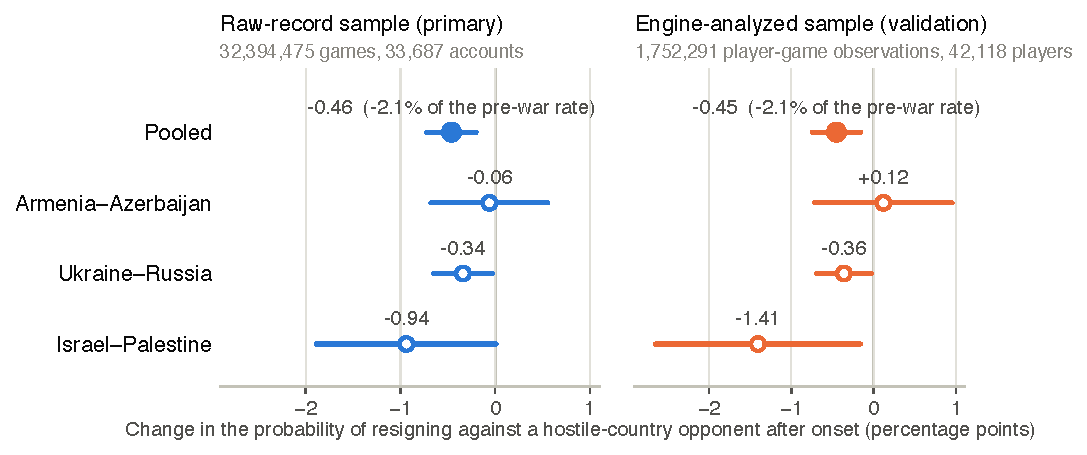
\includegraphics[width=0.56\textwidth]{forest_step3}
  \begin{flushleft}\footnotesize
    \begin{itemize}
      \item Per conflict (raw): Ukraine--Russia $-0.34$ pp (SE 0.16, $p = .031$); Israel--Palestine $-0.94$ pp (SE 0.48, $p = .053$; 4.9\% of its 19.17\% baseline); Armenia--Azerbaijan $-0.06$ pp (SE 0.31, $p = .85$): no change
      \item Engine-analyzed sample, built under different eligibility rules and sampling: $-0.45$ pp (SE 0.15, $p = .0025$), 2.1\% of its 21.80\% baseline; per conflict $-0.36$ ($p = .033$), $-1.41$ ($p = .027$), $+0.12$ ($p = .78$); with each player weighted equally $-1.13$ pp (SE 0.39, $p = .0038$), about 2.5 times its per-game estimate
      \item Leave-one-conflict-out: negative throughout; dropping Ukraine--Russia removes 44\% of observations and roughly doubles the standard error
    \end{itemize}
  \end{flushleft}
  \links{\bk{bk-loo}{leave-one-conflict-out} \quad \hyperlink{corroboration}{\textcolor{linkblue}{\scriptsize\textsf{back: corroboration}}}}
\end{frame}

\begin{frame}[label=bk-composition-full]{Backup: all endings, draws, and game length}
  \centering
  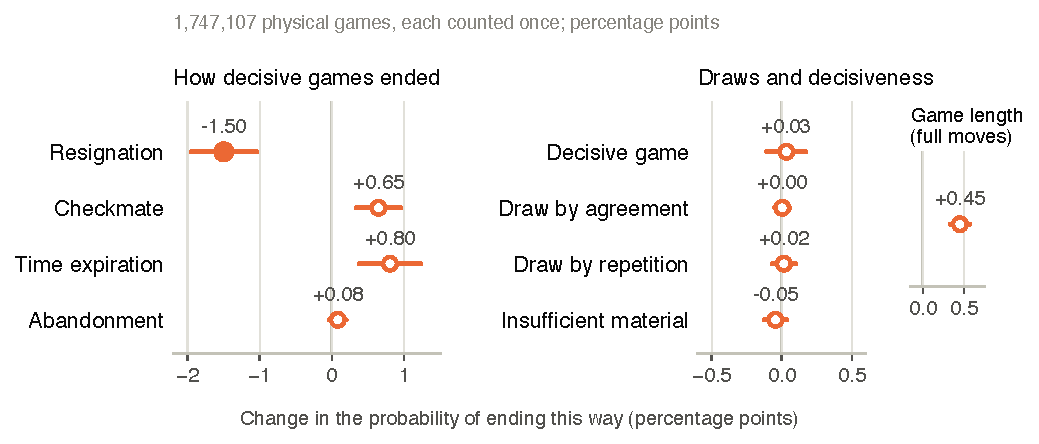
\includegraphics[width=0.52\textwidth]{composition}
  \begin{flushleft}\footnotesize
    \begin{itemize}
      \item Each physical game counted once (1,747,107 games): resignation endings $-1.50$ pp (SE 0.23, $p < .0001$); checkmate $+0.65$ (SE 0.16, $p < .0001$); time expiration $+0.80$ (SE 0.22, $p = .0002$); abandonment $+0.08$ ($p = .16$)
      \item Decisiveness and every kind of draw unchanged. The two increases sum to $+1.45$ pp against the $-1.50$ decline: games that would have ended in concession ran on to checkmate or until a clock ran out
      \item Games slightly longer ($+0.449$ moves), a compositional consequence of fewer early concessions. The estimates record where the endings moved, not why
    \end{itemize}
  \end{flushleft}
  \links{\bk{bk-gamelevel}{game-level estimation} \quad \hyperlink{endings}{\textcolor{linkblue}{\scriptsize\textsf{back: how games ended}}}}
\end{frame}

\begin{frame}[label=bk-persistence-full]{Backup: all persistence measures}
  \begin{columns}[T]
    \begin{column}{0.36\textwidth}
      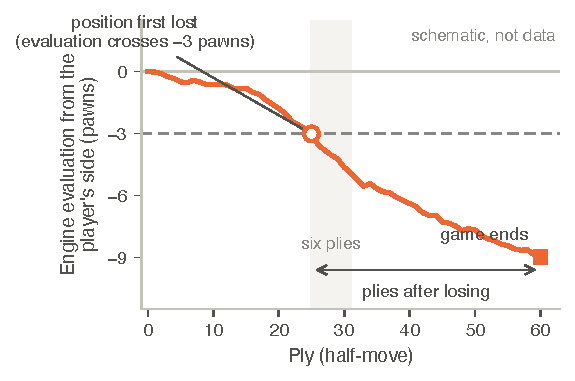
\includegraphics[width=0.92\textwidth]{eval_schematic}
    \end{column}
    \begin{column}{0.64\textwidth}
      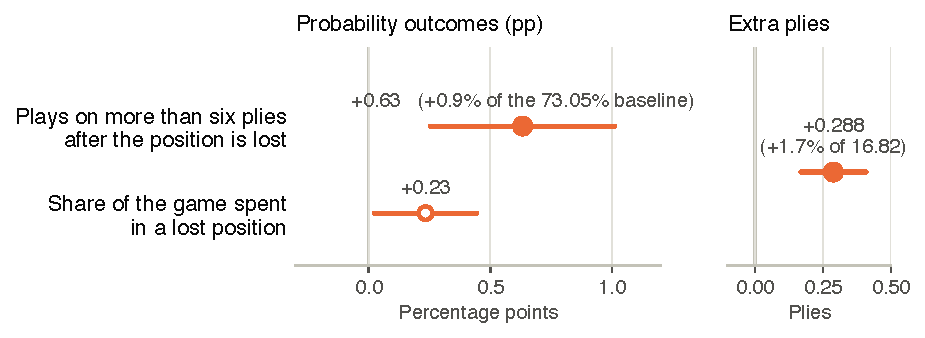
\includegraphics[width=0.92\textwidth]{persistence_main}
    \end{column}
  \end{columns}
  \footnotesize
  \begin{itemize}
    \item Risk set: games in which the player's position ever fell to a disadvantage of three pawns or worse by the engine's contemporaneous evaluation (almost always decisive); membership never depends on the game's result. 1,115,113 player-game observations, 35,925 players
    \item After onset, players played on for $+0.288$ additional plies per lost game (SE 0.061, $p < .0001$) on a pre-conflict mean of 16.82, a 1.7\% increase; more likely to continue beyond six plies, $+0.63$ pp (SE 0.19, $p = .0011$) on 73.05\%; share of the game spent lost $+0.23$ pp (SE 0.11, $p = .030$)
    \item The cost falls on the persister: time and effort in positions offering essentially no prospect of reward
  \end{itemize}
  \links{\bk{bk-persistconflict}{by conflict} \quad \fq{faq-glossary}{plies, pawns, centipawns} \quad \hyperlink{persistence}{\textcolor{linkblue}{\scriptsize\textsf{back: persistence}}}}
\end{frame}

\begin{frame}[label=bk-quality-full]{Backup: three measures of play quality}
  \centering
  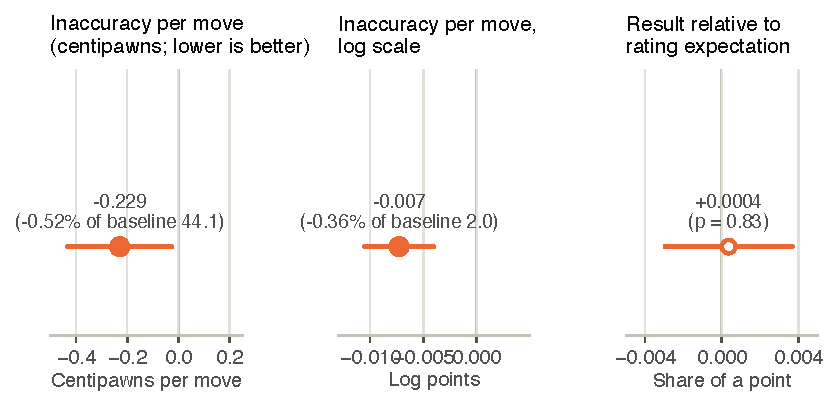
\includegraphics[width=0.58\textwidth]{quality}
  \begin{flushleft}\footnotesize
    \begin{itemize}
      \item Average centipawn loss, the engine's per-move measure of inaccuracy in hundredths of a pawn: $-0.229$ (SE 0.104, $p = .027$); its log-scaled version $-0.0073$ (SE 0.0017, $p < .001$)
      \item Performance relative to the score expected from the rating difference: $+0.0004$ ($p = .83$)
      \item This bounds the readings of persistence: whatever kept players in lost positions, it was not accompanied by deteriorating play
    \end{itemize}
  \end{flushleft}
  \links{\bk{bk-secondary}{full quality and secondary outcomes} \quad \fq{faq-worseplay}{could it be worse play rather than choice?} \quad \hyperlink{quality}{\textcolor{linkblue}{\scriptsize\textsf{back: move quality}}}}
\end{frame}

\begin{frame}[label=bk-openings-full]{Backup: openings by colour, and without Armenia--Azerbaijan}
  \begin{columns}[T]
    \begin{column}{0.56\textwidth}
      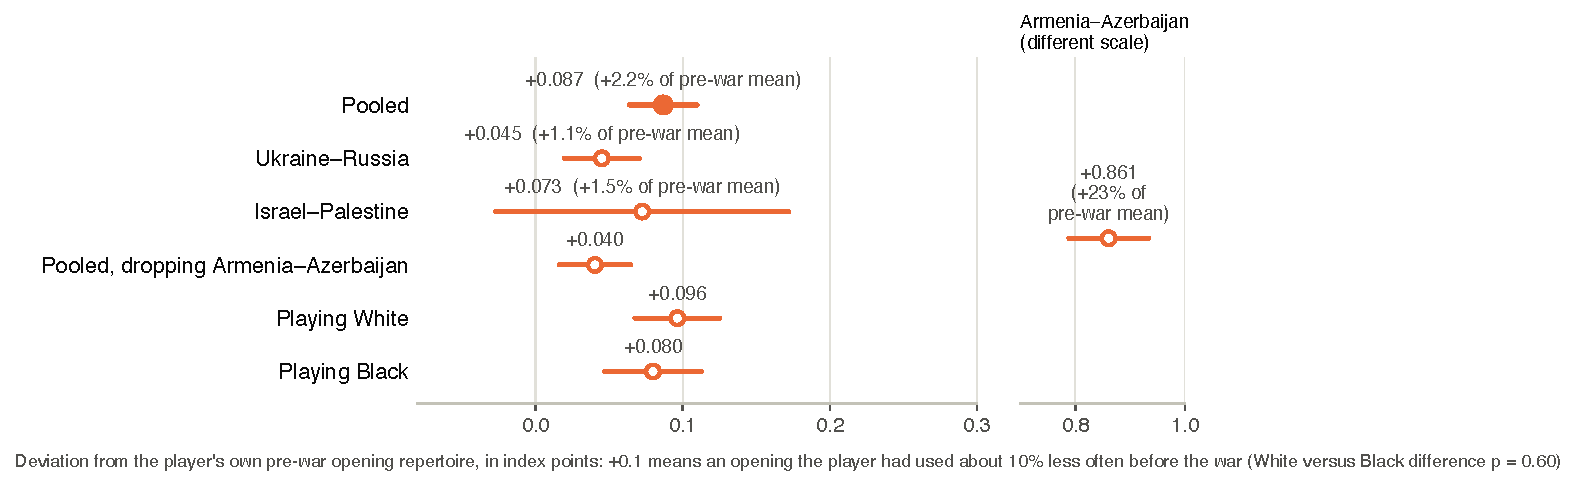
\includegraphics[width=\textwidth]{openings}
    \end{column}
    \begin{column}{0.44\textwidth}
      \footnotesize
      \begin{itemize}
        \item Each opening is scored against the player's own repertoire frozen before onset: minus the log of how often they had used it, so $+0.1$ means an opening used about 10\% less often before the war
        \item Hostile-country games after onset: $+0.0868$ (SE 0.0117, $p < .0001$), 2.2\% of the pre-war mean; White and Black alike ($p = .60$)
        \item Armenia--Azerbaijan drives much of it ($+0.861$); Ukraine--Russia $+0.045$; Israel--Palestine $+0.073$ ($p = .15$); without Armenia--Azerbaijan $+0.040$ ($p = .0011$)
        \item Not sharper play: the aggressive-opening share moved $-0.23$ pp ($p = .069$), the safe-opening share $-0.04$ pp ($p = .82$)
      \end{itemize}
    \end{column}
  \end{columns}
  \links{\bk{bk-openings}{construction of the deviation index} \quad \bk{bk-secondary}{opening-style outcomes} \quad \hyperlink{openings}{\textcolor{linkblue}{\scriptsize\textsf{back: openings}}}}
\end{frame}

\begin{frame}[label=bk-speccurve-full]{Backup: the specification curve with the choice matrix}
  \centering
  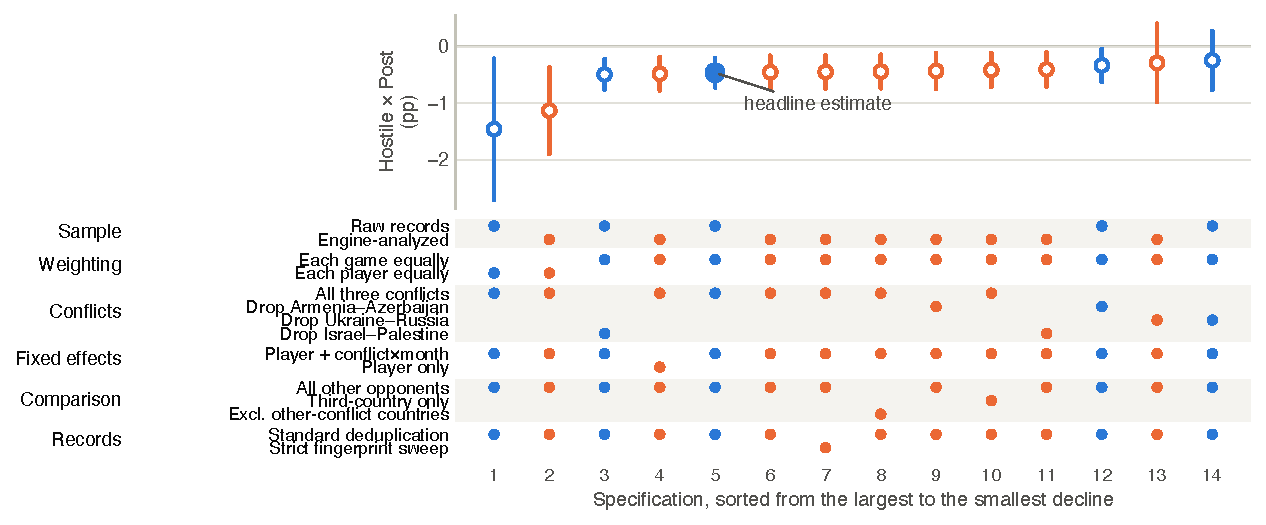
\includegraphics[width=0.63\textwidth]{spec_curve}
  \begin{flushleft}\footnotesize
    \begin{itemize}
      \item Fourteen already-reported specifications of the pooled Hostile $\times$ Post estimate; every one negative. The two widest intervals drop Ukraine--Russia, the largest conflict; the two furthest left are the player-weighted estimands
      \item Stricter deduplication moves the engine estimate from $-0.453$ to $-0.447$ pp; player-only fixed effects give $-0.479$; comparison-group variants $-0.41$ and $-0.44$ pp; clustering by player is the most conservative of four schemes
    \end{itemize}
  \end{flushleft}
  \links{\bk{bk-loo}{leave-one-out} \quad \bk{bk-robust}{robustness dimensions} \quad \hyperlink{sensitivity}{\textcolor{linkblue}{\scriptsize\textsf{back: sensitivity}}}}
\end{frame}

\begin{frame}[label=anyone]{Backup: is anyone driving it?}
  \begin{columns}[T]
    \begin{column}{0.56\textwidth}
      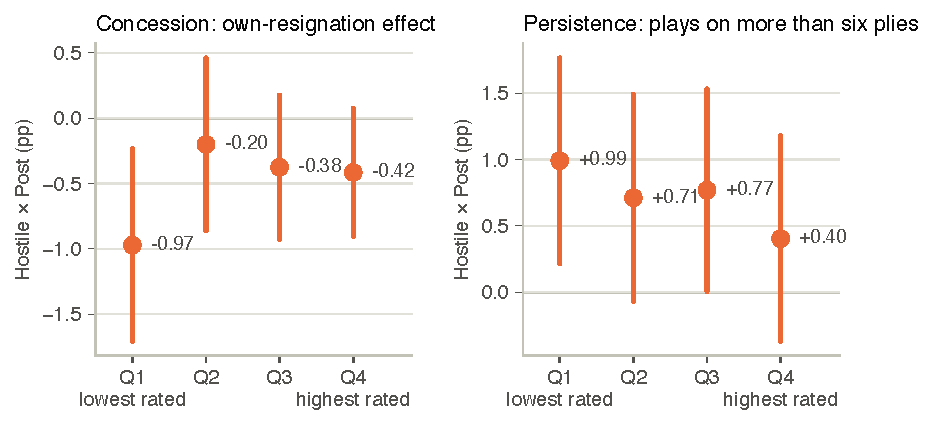
\includegraphics[width=0.92\textwidth]{rating_quartiles}
      {\scriptsize\textcolor{gray}{By quartile of pre-onset rating (engine sample); Hostile $\times$ Post in percentage points with 95\% intervals.}}
    \end{column}
    \begin{column}{0.44\textwidth}
      \footnotesize
      \begin{itemize}
        \item Player-level contrasts for the 8,408 players observed in all four design cells: their spread is fully explained by sampling noise (between-player SD of true effects estimated at zero; about 1.9 pp among the 4,263 best-measured players)
        \item Individual contrasts are noisy (median sampling SE about 27 pp): only the aggregate dispersion is interpretable
        \item Rating: largest in the lowest-rated quartile ($-0.97$ pp, $p = .010$), same direction as persistence, but lowest minus highest is not significant ($p = .22$)
        \item A broad, small shift along the activity margin, not a radical minority
      \end{itemize}
    \end{column}
  \end{columns}
  \links{\bk{bk-dispersion}{dispersion analysis} \quad \bk{bk-rating}{rating quartiles} \quad \fq{faq-heterogeneity}{why no player-level claims?} \quad \hyperlink{whoseaverage}{\textcolor{linkblue}{\scriptsize\textsf{back: whose average}}}}
\end{frame}

\begin{frame}[label=bk-lit1]{Backup: what we know, conflict and parochialism}
  \footnotesize
  \begin{itemize}
    \item People exposed to war become more cohesive within their own group, and their preferences turn parochial, with greater favour toward the in-group rather than greater hostility toward outsiders. The evidence comes from experimental games and surveys among affected populations (Bauer et al.\ 2016; Bauer, Cassar, Chytilov\'a and Henrich 2014).
    \item Perceived threat from ethnic outsiders and sectarian conflict shape cooperation and aggression in local settings (Schaub 2017; Silva and Mace 2014).
    \item Economists have measured the residue of conflict on the sports field. Footballers from countries with a longer history of civil war collect more cards for violent play in European leagues (Miguel, Saiegh and Satyanath 2011). Shared national experiences, such as a national team's victories, strengthen national identification and reduce violence (Depetris-Chauvin, Durante and Campante 2020).
    \item The form of contact matters: collaborative contact across caste lines builds cross-group ties, while adversarial contact erodes them (Lowe 2021). External threat can also shift identity, as Russia's 2014 invasion did for European identification in Ukraine (Gehring 2022).
    \item Nearly all of this measures attitudes, allocations, or aggregates. Almost none of it observes how an individual treats an identifiable member of the adversary.
  \end{itemize}
  \backto{motivation}{motivation}
\end{frame}

\begin{frame}[label=bk-lit2]{Backup: what we know, markets, institutions, expression}
  \footnotesize
  \begin{itemize}
    \item Interstate tension redirects economic exchange. Firms exposed to the other country lost market value during Sino-Japanese diplomatic shocks (Fisman, Hamao and Wang 2014), and political conflict triggers consumer boycotts that cut trade (Heilmann 2016). Consumption itself expresses identity (Atkin, Colson-Sihra and Shayo 2021).
    \item Institutional decision-makers show the same pattern: enforcement of foreign claims in Russian courts fell after 2014 (Shchetinin and Avdeev 2026), the closest institutional analogue to the behaviour studied here.
    \item Online, solidarity and hostility rose on social media around the 2022 invasion of Ukraine (Kyrychenko et al.\ 2024). Expression, however, is addressed to an audience; a game is played against one particular person, in real time, and only one of them can win.
    \item Three gaps. The evidence captures generalized preferences rather than behaviour aimed at an identifiable member of the opposing nation. It is collected in or near war zones, where hostility cannot be told apart from direct experience of violence. And it rarely benchmarks behaviour against an objective measure of the situation.
  \end{itemize}
  \backto{motivation}{motivation}
\end{frame}

% ---------------- Sampling and data

\begin{frame}[label=bk-eligibility]{Backup: eligibility rules for the engine-analyzed sample}
  \small
  \begin{itemize}
    \item A player is eligible with more than 10 games against hostile-country opponents and more than 100 games in total over the combined pre- and post-onset window, after dropping games whose move record was missing
    \item For each eligible player: every hostile-country game is retained, plus a simple random sample of non-hostile games equal to twice the number of hostile games (or all such games if fewer were available), unstratified by period or game characteristics
    \item Result: 1,752,291 player-game observations from 42,118 players covering 1,405,530 physical games
    \item Because eligibility is defined over the full window, it conditions on post-onset play. Participation and attrition are therefore examined in the unrestricted data, and the restricted sample is used only for engine-based outcomes
    \item The raw-record sample has no such restriction: every available game of each sampled account
    \item A small number of games failed engine analysis, most likely games of the Chess960 variant, which starts from a randomized position; no failure log was kept
  \end{itemize}
  \backto{samples}{two samples}
\end{frame}

\begin{frame}[label=bk-frame]{Backup: the sampling frame and the probability-sample caveat}
  \small
  \begin{itemize}
    \item The account database was assembled incrementally since 2018: an initial scrape of a broad list of recently active players, expanded by adding every opponent of each player whose game history was collected. This is a snowball frame: the set of known accounts grows through the games of accounts already known
    \item For each conflict, accounts flagged to the belligerent countries were selected at random from the database, without conditioning on their game histories
    \item Consequence: neither sample is a probability sample of the platform's user base, and the paper makes no claims about how common the behaviour is among chess players, let alone the public
    \item Why the estimand does not need one: the question is whether the same person, facing the same kind of opponent, behaves differently once the countries are at war. A within-person change of that kind is identified without representativeness. Representativeness would matter for a prevalence claim, which is not made
    \item Chess players are a selected population: people who chose competitive play online. The virtues of the setting (scale, objectivity, distance from the battlefield) are also the bounds of what it can represent
  \end{itemize}
  \backto{records}{the records}
\end{frame}

\begin{frame}[label=bk-flags]{Backup: flag-stability audit (re-scrape, September 2024)}
  \centering
  \footnotesize
  \begin{tabular}{@{}lrrrr@{}}
    \toprule
    Country & Accounts & Any change (\%) & Switch rate vs.\ overall & Net flag-to-flag (\%) \\
    \midrule
    All countries & 3,602,092 & 6.03 & 1.00 & 0.00 \\
    Armenia & 15,679 & 4.67 & 0.76 & $+3.08$ \\
    Azerbaijan & 16,812 & 4.80 & 0.59 & $+1.15$ \\
    Russia & 175,459 & 8.99 & 2.12 & $-5.32$ \\
    Ukraine & 53,776 & 6.09 & 0.96 & $+0.94$ \\
    Israel & 26,674 & 6.78 & 1.40 & $+1.19$ \\
    Palestine & 3,477 & 8.37 & 1.92 & $+48.35$ \\
    \bottomrule
  \end{tabular}
  \vspace{2mm}
  \begin{flushleft}\footnotesize
    \begin{itemize}
      \item Displayed flags re-scraped in September 2024 against the collection-era baseline: 94.0\% of accounts carry the same flag (3,384,894 of 3,602,092)
      \item Russia and Palestine are the outliers; the Palestinian inflow (of a small base) is an opponent-classification caveat for the Israel--Palestine conflict only
      \item Misclassification mixes untreated games into the treated set and attenuates the directed estimates toward zero
    \end{itemize}
  \end{flushleft}
  \backto{flags}{flags and selection}
\end{frame}

\begin{frame}[label=bk-flagmeaning]{Backup: what a displayed flag is, and is not}
  \begin{itemize}
    \item The flag is the account's displayed profile country: a self-reported signal, which the user can change at any time. The platform assigns a default at account creation based on location; this platform-policy detail is to be verified against the live page before it enters the manuscript
    \item Focal players were sampled on their pre-conflict flags, so sampling cannot respond to the war
    \item A displayed flag is never citizenship, and the two are never equated. Analysis language stays dyad-neutral: ``hostile-country opponent'' means the displayed-country definition throughout
    \item Stability: 94.0\% of accounts carried the same flag between collection and the September 2024 re-scrape; the exception with teeth is the inflow into the Palestinian flag
    \item Direction of any error: mixing untreated games into the treated set attenuates the directed estimates toward zero, so misclassification works against finding an effect
  \end{itemize}
  \backto{flags}{flags and selection}
\end{frame}

\begin{frame}[label=bk-table1]{Backup: how Table 1 counts games, observations and accounts}
  \small
  \begin{itemize}
    \item Three counts are reported separately throughout: player-game observations (the regression N), physical games, and focal accounts
    \item A player-game observation is one focal player's perspective on one game. Nearly every hostile physical game between two sampled players appears twice, once from each side, so own- and opponent-side coefficients are mechanically linked and are never presented as independent findings
    \item Physical games are deduplicated on the game's identifying keys (date, start and end time, opening code, termination). A game whose two players belong to different conflict samples is counted in both per-conflict rows and once in the pooled row, so the per-conflict physical-game column sums above the pooled total
    \item The pooled sample is dyad-restricted: a focal player enters only through the sample of their own conflict
    \item Clean game-level quantities (composition of endings, game length) are estimated once per physical game, with the alphabetically first player's perspective retained as a tie-break: 1,747,107 games, 54,904 retained perspectives
  \end{itemize}
  \backto{bk-table1-main}{the three conflicts}
\end{frame}

\begin{frame}[label=bk-2014]{Backup: the Ukraine--Russia 2014 robustness sample}
  \small
  \begin{itemize}
    \item 1,173 accounts; 1,187,263 physical games; 1,276,315 player-game observations; onset 20 February 2014
    \item Excluded from pooling: a different platform era and data density; used for robustness only
    \item Own-resignation, raw records: $+0.18$ pp (SE 0.67, $p = .78$); engine-analyzed sample $-0.72$ pp (SE 0.79, $p = .37$). Resignation endings of either kind, raw: $-1.88$ pp (SE 0.77, $p = .014$)
    \item Persistence: plays on beyond six plies $+2.38$ pp (SE 1.04, $p = .023$); the largest of the per-conflict persistence estimates
    \item Openings: deviation from the frozen repertoire $+0.463$ (SE 0.059, $p < .0001$)
    \item Limitation, stated wherever the sample appears: the binned pre-onset test for resignation endings of either kind rejects at the 5\% level ($p = .0197$); for own-resignation it does not ($p = .137$)
  \end{itemize}
  \backto{bk-table1-main}{the three conflicts}
\end{frame}

% ---------------- Specification

\begin{frame}[label=bk-robust]{Backup: robustness dimensions tested}
  \centering
  \scriptsize
  \setlength{\tabcolsep}{3pt}
  \begin{tabular}{@{}p{0.2\textwidth}p{0.42\textwidth}p{0.33\textwidth}@{}}
    \toprule
    Dimension & What was varied & Pooled own-resignation estimate \\
    \midrule
    Sample & Raw records versus the engine-analyzed sample (independent construction) & $-0.46$ versus $-0.45$ pp \\
    Weighting & Each game versus each player equally & $-0.46$ versus $-1.46$ pp (raw); $-0.45$ versus $-1.13$ (engine) \\
    Conflicts & Leave one conflict out & $-0.33$ (no AA), $-0.49$ (no IL--PS), $-0.24$ pp (no UA--RU; imprecise) \\
    Fixed effects & Player only, without conflict-by-month effects & $-0.479$ versus $-0.453$ pp (engine) \\
    Comparison group & Third-country opponents only; excluding other-conflict countries & $-0.41$ ($p = .0072$); $-0.44$ pp ($p = .0036$) \\
    Duplicate records & Strict full-field fingerprint sweep (3,057 rows removed) & $-0.453$ to $-0.447$ pp \\
    Clustering & Player; physical game; two-way; unordered pair & SE 0.001496 by player is the largest of the four \\
    Engine-sample repair & Omitted hostile games re-collected for about 30\% of engine-sample players & Magnitudes attenuated 1.5--10\%; inference unchanged; raw sample unaffected \\
    Onset timing & Excluding the partial onset month & Reported in the SI \\
    \bottomrule
  \end{tabular}
  \backto{sensitivity}{sensitivity}
\end{frame}

\begin{frame}[label=bk-gamelevel]{Backup: game-level estimation}
  \begin{itemize}
    \item Composition outcomes (how games ended, game length) are estimated once per physical game, which removes the mechanical duplication of player-game rows
    \item Where both players of a game were sampled, the alphabetically first player's perspective is retained as a tie-break: 1,747,107 games with 54,904 retained perspectives
    \item The specification keeps sample-by-month effects and both players' ratings but no player effects (a game no longer belongs to one focal player), and clusters standard errors on the retained perspective
    \item Outcomes: endings by resignation, checkmate, time expiration, abandonment; decisiveness; the three draw types; and game length in full moves
    \item These estimates complement, and are never independent of, the directed results: a directed own-resignation and its mirror, opponent-resignation, are two sides of the same physical game
  \end{itemize}
  \backto{endings}{how games ended}
\end{frame}

% ---------------- Dynamics

\begin{frame}[label=bk-monthly]{Backup: monthly event study, raw-record sample}
  \centering
  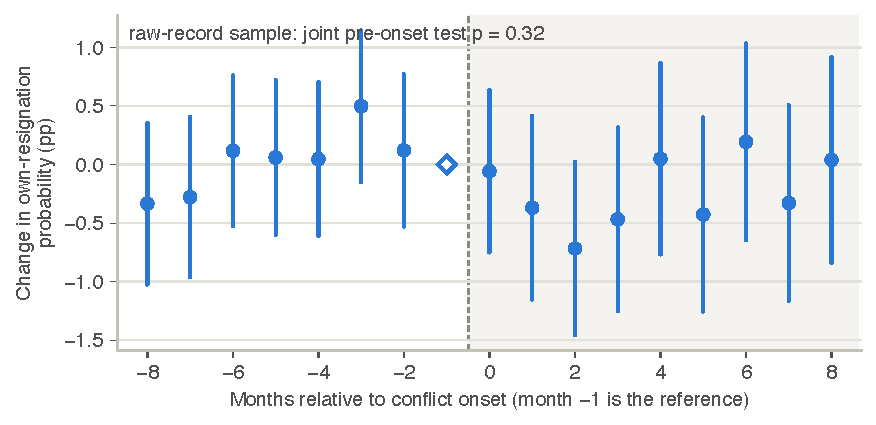
\includegraphics[width=0.72\textwidth]{event_monthly_raw}
  \begin{flushleft}\footnotesize
    Months $-8$ to $+8$ around onset; player and sample-by-month effects; the joint chi-squared test on all pre-onset leads gives $p = .320$.
  \end{flushleft}
  \backto{before}{before onset}
\end{frame}

\begin{frame}{Backup: monthly event study, engine-analyzed sample}
  \centering
  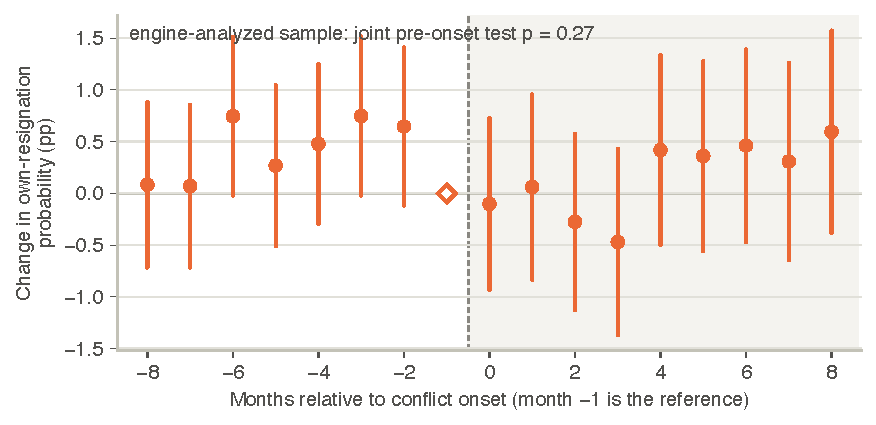
\includegraphics[width=0.72\textwidth]{event_monthly_engine}
  \begin{flushleft}\footnotesize
    Same specification on the engine-analyzed sample; the joint pre-onset test gives $p = .266$.
  \end{flushleft}
  \backto{before}{before onset}
\end{frame}

\begin{frame}[label=bk-fullwindow]{Backup: three-month bins to month 17}
  \centering
  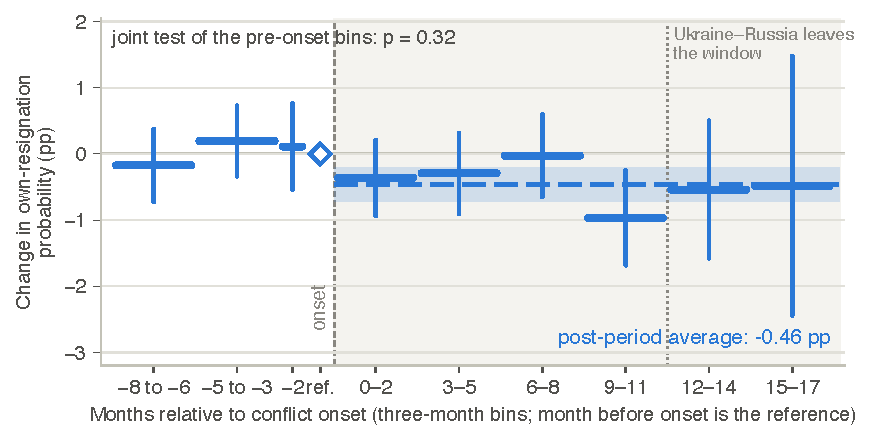
\includegraphics[width=0.7\textwidth]{event_full_window}
  \begin{flushleft}\footnotesize
    The bins for months 12--14 ($-0.54$ pp) and 15--17 ($-0.48$ pp) are negative but imprecise. Ukraine--Russia, the largest sample, exits the window after month 11, so these bins rest on the remaining conflicts alone, and even the 9--11 bin draws on fewer Ukraine--Russia months.
  \end{flushleft}
  \backto{after}{after onset}
\end{frame}

\begin{frame}[label=bk-pretrends]{Backup: joint pre-onset tests by conflict}
  \centering
  \small
  \begin{tabular}{@{}lrrr@{}}
    \toprule
    Own-resignation & Raw, binned & Raw, monthly & Engine, monthly \\
    \midrule
    Pooled & .316 & .320 & .266 \\
    Armenia--Azerbaijan & .825 & .613 & .685 \\
    Ukraine--Russia 2022 & .332 & .353 & .305 \\
    Israel--Palestine & .378 & .504 & .452 \\
    Ukraine--Russia 2014 & .137 & .381 & .038 \\
    \bottomrule
  \end{tabular}
  \begin{flushleft}
    \begin{itemize}
      \item $p$-values of the joint chi-squared test on all pre-onset coefficients (month $-1$ omitted)
      \item No test rejects at the 5\% level in the three pooled conflicts. The 2014 robustness sample rejects in the engine monthly version, and its binned test for resignation endings of either kind rejects ($p = .0197$); this limitation is noted wherever that sample appears
    \end{itemize}
  \end{flushleft}
  \backto{before}{before onset}
\end{frame}

\begin{frame}[label=bk-contact]{Backup: Ukraine--Russia, contact with the other side month by month}
  \centering
  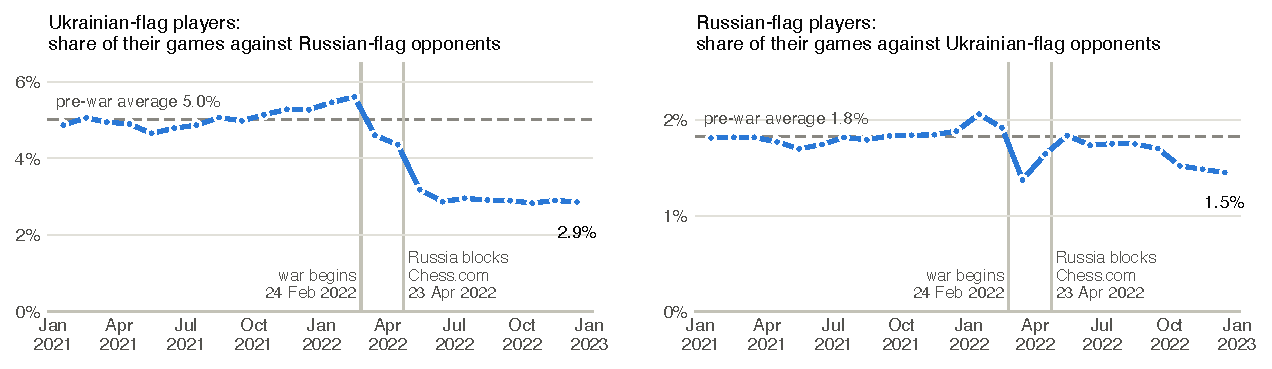
\includegraphics[width=0.9\textwidth]{contact_by_month}
  \begin{flushleft}\footnotesize
    \begin{itemize}
      \item No drop at onset. The Ukrainian-side share steps down in May, the first full month after Russia blocked the platform; the Russian-side share dips in March and is back at its pre-war level from May to September
      \item A game left before the first move vanishes from both players' records, so avoidance would lower both series together. They move apart, which points to the supply of opponents; avoidance cannot be excluded
    \end{itemize}
    {\scriptsize\textcolor{gray}{Monthly counts from the full raw records (first results, not yet in the paper).}}
  \end{flushleft}
  \links{\fq{faq-quit}{quit on seeing the flag?} \quad \fq{faq-avoid}{can players avoid opponents?} \quad \hyperlink{flags}{\textcolor{linkblue}{\scriptsize\textsf{back: limitations}}}}
\end{frame}

% ---------------- Persistence, quality, openings

\begin{frame}[label=bk-persistconflict]{Backup: persistence by conflict}
  \centering
  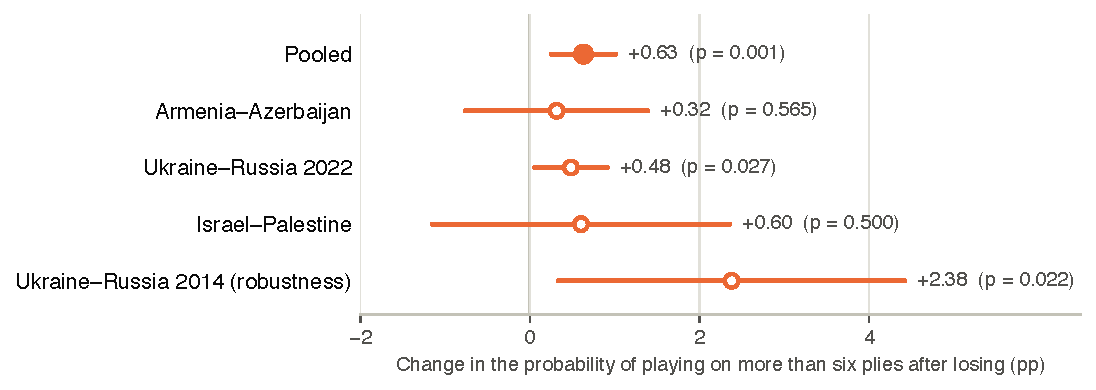
\includegraphics[width=0.74\textwidth]{persistence_by_conflict}
  \begin{flushleft}\footnotesize
    Probability of continuing more than six plies after the position first became lost; player and conflict-by-month effects; 95\% confidence intervals. Positive in all four samples and statistically powered in the largest.
  \end{flushleft}
  \backto{checks}{checks}
\end{frame}

\begin{frame}[label=bk-secondary]{Backup: play-quality and secondary outcomes (engine-analyzed sample, pooled)}
  \centering
  \footnotesize
  \begin{tabular}{@{}lrrr@{}}
    \toprule
    Outcome & Estimate & SE & $p$ \\
    \midrule
    Average centipawn loss (centipawns) & $-0.229$ & 0.104 & .027 \\
    Average log centipawn loss (log points) & $-0.0073$ & 0.0017 & $< .001$ \\
    Overperformance vs.\ rating expectation (score share) & $+0.0004$ & 0.0017 & .83 \\
    \midrule
    Aggressive opening (pp) & $-0.23$ & 0.12 & .069 \\
    Safe opening (pp) & $-0.04$ & 0.18 & .82 \\
    Ended on time (pp) & $+0.23$ & 0.17 & .16 \\
    Draw by repetition (pp) & $+0.10$ & 0.05 & .046 \\
    Draw by agreement (pp) & $+0.02$ & 0.03 & .48 \\
    Insufficient material (pp) & $+0.04$ & 0.05 & .45 \\
    Abandonment (pp) & $+0.09$ & 0.06 & .10 \\
    Stalling (pp) & $+0.06$ & 0.07 & .36 \\
    \bottomrule
  \end{tabular}
  \begin{flushleft}\footnotesize
    Hostile $\times$ Post; player-game observations; player and conflict-by-month effects; clustered by player.
  \end{flushleft}
  \backto{quality}{move quality}
\end{frame}

\begin{frame}[label=bk-openings]{Backup: the repertoire-deviation index}
  \begin{itemize}
    \item The opening is the first phase of a game, when players choose among well-known sequences of moves; most settle on a small set of favourites (their repertoire) and reach for it by habit
    \item Each game's opening is scored against the player's own pre-conflict repertoire: the repertoire is frozen before onset and scored out of sample within the pre-period, with smoothing applied evenly across openings
    \item Higher values mean the game's opening was rarer in that player's own pre-war play; the index measures deviation from habit, not preparation and not identity
    \item Freezing the repertoire before onset matters: scoring each game against a whole-period repertoire would let post-onset games partly define their own familiarity
    \item Symmetry across colours (White $+0.096$, Black $+0.080$, difference $p = .60$) rules out an artifact of White choosing the opening
    \item Scoring variants are reported in the SI
  \end{itemize}
  \backto{openings}{openings}
\end{frame}

\begin{frame}[label=bk-aalength]{Backup: game length in Armenia--Azerbaijan}
  \small
  \begin{itemize}
    \item Before the war, hostile-country games in this dyad were already longer than the same players' other games: mean length 37.43 moves versus 35.12 (raw-record sample, pre-onset)
    \item Game length after onset (Hostile $\times$ Post, engine-analyzed sample, full moves):
  \end{itemize}
  \centering
  \begin{tabular}{@{}lrrr@{}}
    \toprule
    Group & Estimate & SE & $p$ \\
    \midrule
    Pooled & $+0.437$ & 0.055 & $< .0001$ \\
    Armenia--Azerbaijan & $+0.527$ & 0.168 & .0018 \\
    Ukraine--Russia 2022 & $+0.225$ & 0.061 & .0003 \\
    Israel--Palestine & $+0.564$ & 0.236 & .017 \\
    \bottomrule
  \end{tabular}
  \begin{flushleft}
    \begin{itemize}
      \item Game length is a secondary compositional consequence of fewer early concessions, not a separate finding; the pre-existing gap in this dyad is stated alongside the null on resignation
    \end{itemize}
  \end{flushleft}
  \backto{boundary}{the boundary}
\end{frame}

% ---------------- Heterogeneity and other

\begin{frame}[label=bk-dispersion]{Backup: dispersion of player-level effects}
  \centering
  \footnotesize
  \begin{tabular}{@{}lrrrr@{}}
    \toprule
    Players included & N & Weighted mean & SD of true effects & Dispersion test \\
    \midrule
    All four design cells occupied & 8,408 & $-0.56$ pp & 0.0 pp & $Q = 8{,}328$ on 8,407 df \\
    At least five games per cell & 4,263 & $-0.51$ pp & 1.9 pp & $Q = 4{,}450$ on 4,262 df \\
    \bottomrule
  \end{tabular}
  \begin{flushleft}
    \begin{itemize}
      \item Each player's own difference-in-differences contrast on own-resignation, with a binomial sampling variance smoothed so that empty cells do not yield zero variance; an empirical-Bayes layer tests whether the spread exceeds what sampling variances alone would produce (DerSimonian--Laird)
      \item In the full set, the observed spread is fully explained by sampling noise; in the better-measured half, the estimated spread of true effects is about 1.9 pp around a mean of about $-0.5$ pp
      \item The per-player contrasts net out player-level time shifts through the player's own other games but do not impose the headline specification's conflict-by-month effects; the analysis is descriptive
      \item The four-cell requirement selects the most active players; less active players are unmeasurable at the player level by construction
    \end{itemize}
  \end{flushleft}
  \backto{whoseaverage}{whose average}
\end{frame}

\begin{frame}[label=bk-rating]{Backup: rating quartiles, concession and persistence}
  \centering
  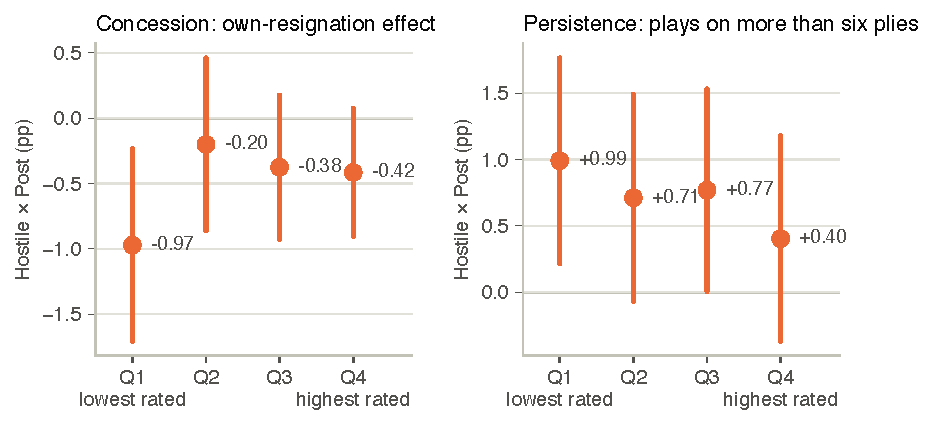
\includegraphics[width=0.7\textwidth]{rating_quartiles}
  \begin{flushleft}\footnotesize
    Players assigned to quartiles of pre-onset mean rating within their conflict sample; headline specification by quartile. Concession: lowest minus highest $-0.56$ pp ($p = .22$). Both gradients point the same way but neither cross-quartile difference is significant; descriptive only.
  \end{flushleft}
  \backto{whoseaverage}{whose average}
\end{frame}

\begin{frame}[label=bk-activity]{Backup: activity quartiles and the pooled trend test}
  \centering
  \footnotesize
  \begin{tabular}{@{}lrrrrr@{}}
    \toprule
    Quartile (pre-onset hostile games) & Estimate (pp) & SE & $p$ & Players & Rel.\ to baseline \\
    \midrule
    Q1 least active & $-1.73$ & 1.36 & .20 & 3,753 & $-7.2\%$ \\
    Q2 & $-1.18$ & 0.88 & .18 & 11,323 & $-5.0\%$ \\
    Q3 & $-0.57$ & 0.47 & .23 & 11,833 & $-2.4\%$ \\
    Q4 most active & $-0.35$ & 0.17 & .035 & 11,834 & $-1.6\%$ \\
    \bottomrule
  \end{tabular}
  \begin{flushleft}
    \begin{itemize}
      \item Q1 minus Q4: $-1.38$ pp ($p = .31$); the least active quartile carries the least data by construction
      \item Pooled interaction of Hostile $\times$ Post with standardized log activity: $+0.06$ pp per SD ($p = .58$); that regression is game-weighted, so it is dominated by the active players it is trying to contrast
      \item Even the least active players clear the engine sample's eligibility floor of more than 10 hostile-country games, so the range is compressed
    \end{itemize}
  \end{flushleft}
  \backto{whoseaverage}{whose average}
\end{frame}

\begin{frame}[label=bk-loo]{Backup: leave-one-conflict-out}
  \centering
  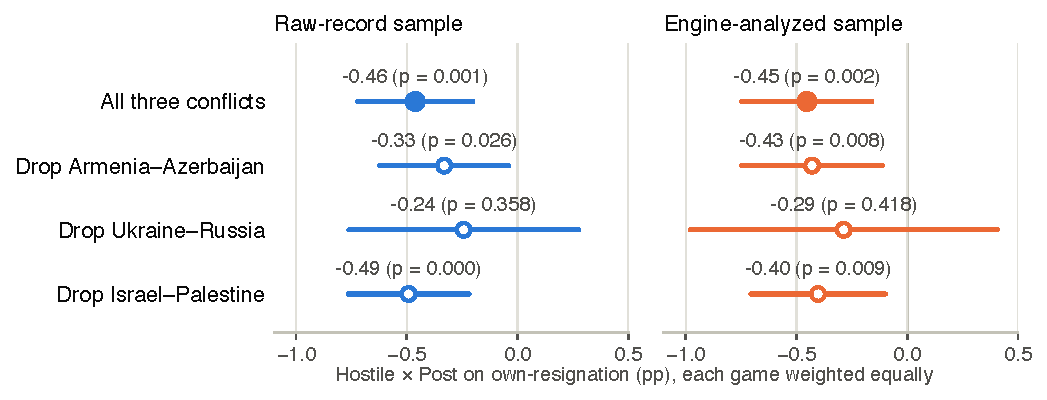
\includegraphics[width=0.74\textwidth]{loo}
  \begin{flushleft}\footnotesize
    Raw records: without Armenia--Azerbaijan $-0.33$ pp (SE 0.15); without Israel--Palestine $-0.49$ pp (SE 0.14); without Ukraine--Russia $-0.24$ pp (95\% CI $-0.76$ to $+0.28$), consistent with both the pooled estimate and zero. Excluding Ukraine--Russia removes 44\% of observations (35.9M to 20.3M); its own per-conflict estimate is independently negative ($-0.34$ pp, $p = .031$).
  \end{flushleft}
  \backto{byconflict}{by conflict}
\end{frame}

\begin{frame}[label=bk-ethics]{Backup: ethics and data governance}
  \begin{itemize}
    \item All data derive from publicly available game records, analyzed at scale with de-identified accounts; no interaction with players and no manipulation
    \item Account names are pseudonymized in the replication release; no cross-linking to off-platform identity was attempted
    \item Displayed country is an inferred, self-reported signal; analysis language remains dyad-neutral, and nationality or citizenship is never asserted
    \item Approved by the University of Queensland Human Research Ethics Committee (approval 2026/HE011640)
    \item Replication code and outputs released at a tagged commit of the project repository; data deposit via the University of Queensland Research Data Manager; the archive may include the raw game records, whose redistribution the platform permits
  \end{itemize}
  \backto{backup-index}{backup index}
\end{frame}

\begin{frame}[label=bk-iran]{Backup: Iran feasibility}
  \begin{itemize}
    \item Onset: February 2026. The September 2024 account re-scrape predates it, so focal players can be sampled on pre-conflict flags, as the design requires
    \item Pool size: about 44,000 Iranian-flagged accounts in the re-scrape, roughly three times the Armenian pool, with no shortage on the other side
    \item The specification (exact onset, dyad restriction, player and conflict-by-month effects, both weightings) was frozen months before any Iranian data were examined; a timestamped pre-analysis plan turns the run into a preregistered out-of-sample replication
    \item Trade-off: running now bakes in whatever a short post-onset window shows, including possibly a noisy null; waiting lengthens the window
  \end{itemize}
  \src{Pool counts from the coauthors' September 2024 re-scrape; not part of the frozen manuscript outputs.}
  \backto{nextsteps}{next steps}
\end{frame}

% =====================================================================
% FAQ
% =====================================================================
\section{FAQ}

\begin{frame}[label=faq-index]{FAQ}
  \footnotesize
  \begin{enumerate}
    \item \hyperlink{faq-lpm}{Why a linear probability model and not a logit?}
    \item \hyperlink{faq-magnitude}{What do $-1.46$ and $-0.46$ percentage points mean concretely?}
    \item \hyperlink{faq-weighting}{Why does weighting players equally triple the estimate?}
    \item \hyperlink{faq-exogenous}{What exactly is exogenous here, and what is not?}
    \item \hyperlink{faq-flags}{Are flags citizenship?}
    \item \hyperlink{faq-aa}{Why is Armenia--Azerbaijan null?}
    \item \hyperlink{faq-heterogeneity}{Why does the paper not claim individual-level heterogeneity?}
    \item \hyperlink{faq-worseplay}{Could the effect be worse play rather than a choice?}
    \item \hyperlink{faq-independent}{Why do the two samples count as independent corroboration?}
    \item \hyperlink{faq-conflicts}{Why these three conflicts?}
    \item \hyperlink{faq-avoid}{Can players avoid hostile-country opponents?}
    \item \hyperlink{faq-structural}{Is there a structural model behind this?}
    \item \hyperlink{faq-glossary}{Glossary: plies, pawns, centipawns, ratings, time controls}
    \item \hyperlink{faq-quit}{Could players simply have quit on seeing the flag?}
    \item \hyperlink{faq-pretrends}{Why should the pre-onset estimates be zero?}
  \end{enumerate}
  \links{\hyperlink{backup-index}{\textcolor{linkblue}{\scriptsize\textsf{backup index}}}}
\end{frame}

\begin{frame}[label=faq-lpm]{FAQ: why a linear probability model and not a logit?}
  \footnotesize
  The outcome is binary (the focal player resigned, or did not), so a logit is the natural alternative. We estimate a linear probability model for two reasons.

  First, interpretability. The coefficient $\beta$ is directly the change in the probability of resigning, in percentage points, which is the unit the whole paper reports and the unit in which the two weightings (per game and per player) can be compared without further transformation.

  Second, tractability. The raw-record sample has 36 million rows with player fixed effects and conflict-by-month effects. A fixed-effects logit at that scale was not run, and with tens of thousands of player effects the nonlinear estimator also faces the incidental-parameters problem.

  The usual objection to the linear model is that fitted probabilities can leave the unit interval. Here that has little bite. The pre-onset resignation rates sit near 0.19 to 0.22, and the estimated effects are fractions of a percentage point. For example, take a player who resigns 21\% of hostile-country games before the war. A decline of half a percentage point moves that to about 20.5\%, nowhere near a boundary. The relative effects the paper reports (about 2\% of the baseline per game, about 7\% for the typical player) are plain ratios of the estimate to the baseline rate; a logit would report odds ratios, a different quantity, and none was estimated.
  \backto{equation}{estimating equation}
\end{frame}

\begin{frame}[label=faq-magnitude]{FAQ: what do $-1.46$ and $-0.46$ percentage points mean concretely?}
  \footnotesize
  Before onset, players resigned 21.46\% of their games against hostile-country opponents. Weighting each player equally, the typical player resigned 1.46 percentage points less often in those games after onset than their own games against everyone else would predict: 6.8\% of the pre-conflict rate. Weighting each game equally, an average dominated by the most active players, the estimate is 0.46 percentage points, 2.1\%.

  The right yardstick is the games a player loses, because a player can resign only a game they are losing. Take 1,000 hostile-country games before the war. The player lost about 460 of them by resignation, checkmate or on time: about 215 by resigning, 108 by checkmate and 135 on time (a few further losses, in abandoned games, are not counted here). Resignation therefore ended about 47\% of these lost games. For the typical player the estimate removes about 15 of the 215 resignations, leaving about 200, or about 44\% of lost games: roughly 3 fewer resignations in every 100 lost games. On the per-game estimate it is about 5 fewer, or about 46\%.

  The losses did not become rarer. In the per-game estimates the player's resignations fell by 0.46 percentage points while losses by checkmate and on time rose by 0.22 and 0.37. The same games were lost; they ended differently.

  The proportional figure does not depend on the yardstick: 15 fewer out of 215 is 6.8\% whether the 215 are set against 1,000 games or 460 lost games. Set against all games, the change is 15 in 1,000, or about one game in seventy (one divided by 0.0146 is roughly 68).
  \backto{headline}{the headline}
\end{frame}

\begin{frame}[label=faq-weighting]{FAQ: why does weighting players equally triple the estimate?}
  \footnotesize
  The two numbers are two estimands, not two estimates of one thing. The game-weighted coefficient is the average change per game; the player-weighted coefficient is the average change per player. They differ whenever the players who change most are not the players who play most.

  A hypothetical example with two players. Player A plays 900 hostile-country games and her resignation rate in those games falls by 0.2 percentage points. Player B plays 100 hostile-country games and his rate falls by 3 percentage points. Weighting each game equally gives $(900 \times 0.2 + 100 \times 3) / 1{,}000 = 0.48$ percentage points. Weighting each player equally gives $(0.2 + 3) / 2 = 1.6$ percentage points, more than three times as large. Nothing about either player changed between the two calculations; only the question did.

  Because the game-weighted estimate weights each player by how much they play, a threefold gap in the actual data means, by construction, that the decline is concentrated among less active players and that the most active players, who supply most of the games, changed least. The descriptive quartile gradient by pre-war activity shows the same shape, though no between-quartile test is significant; the inference rests on the weighting comparison itself, where both estimates are clearly negative.
  \backto{whoseaverage}{whose average}
\end{frame}

\begin{frame}[label=faq-exogenous]{FAQ: what exactly is exogenous here, and what is not?}
  \footnotesize
  Three things are worth separating.

  \textbf{Onset timing.} The treatment is the start of a war between two countries. No chess player's behaviour on the platform determines it, and it arrives at an exact date that is applied identically in both samples.

  \textbf{Pairing.} Conditional on two players both seeking a game at the same moment in the same time control, the platform's matchmaking pairs them by rating proximity and availability, without regard to nationality, and offers no way to filter opponents by country. So within a moment, whether a given opponent is from the hostile country is not the player's choice.

  \textbf{Who is in the pool.} This is not exogenous. Players choose when and whether to play, activity from the belligerent countries changes during a war, and displayed flags can change. Conflict-by-calendar-month effects absorb any such shift that is common to a conflict's players in a month, and the flag audit bounds the last channel. What remains is the formal assumption: absent onset, a player's hostile-versus-other gap would have evolved in parallel. The flat pre-onset bins support it; a dedicated participation and matching diagnostic in the SI examines the pool directly.

  The paper deliberately does not describe pairing as random in an unconditional sense, because the post-onset pool itself changes. The claim is narrower and, we think, more defensible.
  \backto{comparison}{the comparison}
\end{frame}

\begin{frame}[label=faq-pretrends]{FAQ: why should the pre-onset estimates be zero?}
  \footnotesize
  Because the design removes a difference in levels, not a difference in trends, and the pre-onset bins test for a trend.

  Two things could be called a ``pre-onset difference''. The first is the level of the gap: before the war a player resigned hostile-country games slightly less often than their other games (0.25 percentage points, within the same player). That is allowed: the design compares the gap after onset with the gap before, so a gap that is constant over time cancels.

  The second is whether the gap was already changing before the war. That is what the bars show: each is the gap in that three-month bin minus the gap in the month before onset. The design assumes that without the war the gap would have stayed where it was (parallel trends). That cannot be tested after onset, but it implies that the gap was not drifting before onset, which can be: the pre-trends test.

  A hypothetical example. Suppose the gap had been widening by 0.1 percentage points every three months before the war, for unrelated reasons. It would have kept widening afterwards, and comparing after with before would show a decline of several tenths of a point with no war effect at all. Flat pre-onset bins rule that out.

  What we find: the three pre-onset bins are $-0.17$, $+0.20$ and $+0.11$ percentage points. They alternate in sign, show no drift, and are jointly indistinguishable from zero ($p = .32$).

  Two cautions. Failing to reject zero is not proof: each bin is about as precise as a post-onset bin, so a small drift cannot be excluded. And flat bins say nothing about a shock arriving exactly at onset.
  \backto{before}{before onset}
\end{frame}

\begin{frame}[label=faq-flags]{FAQ: are flags citizenship?}
  \footnotesize
  No, and the paper never equates them; but the design is less exposed to this than it first sounds, because focal players were sampled on the flags they displayed before the conflict, so the sample itself cannot respond to the war. The flag is the country displayed on the account's profile. The platform assigns a default at account creation based on the user's location, and the user can change it at any time; that policy detail is to be verified against the live platform page before it enters the manuscript.

  Two facts limit how much this matters. First, stability: re-scraping displayed flags in September 2024 against the collection-era baseline, 94.0\% of accounts carried the same flag across seven years. Russia (a switch rate 2.12 times the overall rate and a net outflow of 5.32\%) and Palestine (1.92 times, and a net inflow of 48.35\% of a small base) are the outliers; the Palestinian inflow is a classification caveat for the Israel--Palestine conflict only. Second, direction: misclassification mixes untreated games into the treated set, which attenuates the directed estimates toward zero. Errors of this kind work against finding an effect.

  What the paper studies is behaviour toward opponents displaying the other belligerent's flag; ``hostile-country opponent'' means exactly that throughout, and the analysis language stays dyad-neutral.
  \backto{bk-hostile}{hostile games}
\end{frame}

\begin{frame}[label=faq-aa]{FAQ: why is Armenia--Azerbaijan null?}
  \footnotesize
  We do not know, and the paper does not claim to. What it reports is the null itself, with the same prominence as the positive results: no change in own-resignation in either sample ($-0.06$ pp, $p = .85$, raw; $+0.12$ pp, $p = .78$, engine-analyzed), alongside a pre-existing tendency for hostile-country games in this dyad to run longer than other games.

  Three readings are open, none tested. First, duration: active hostilities ended with the trilateral ceasefire roughly six weeks after onset, in November 2020, so most of the post-onset window lies outside active fighting. Second, the three wars differ in intensity and in how salient they were to daily life. Third, the samples differ in dyad-specific ways: who plays online, and how countries are displayed.

  Recoding the months after the ceasefire as untreated, or dropping them, leaves only the six weeks of fighting, far too few hostile-country games to estimate anything for this conflict on its own, and it does not strengthen the pooled estimate (an exploratory check, not in the paper).

  What the null does not mean is that nothing happened in this dyad. Armenia--Azerbaijan moves most on a different margin: departures from each player's habitual openings ($+0.861$ index points, against $+0.045$ in Ukraine--Russia). The margin structure is part of the finding, and it is why the paper says ``across three conflicts'' only when this null is stated alongside.

  Conflict duration, intensity, diaspora composition, and platform exposure are named as moderator candidates for future work.
  \backto{boundary}{the boundary}
\end{frame}

\begin{frame}[label=faq-heterogeneity]{FAQ: why does the paper not claim individual-level heterogeneity?}
  \footnotesize
  Because individual players cannot be measured precisely enough. Take one player's own difference-in-differences contrast: the change in their resignation rate in hostile-country games minus the change in their other games. The median player has few hostile-country games, so that contrast has a sampling standard error of about 27 percentage points. A player whose raw contrast is $-40$ percentage points is about one standard error from zero; the number says almost nothing about that player. Reporting the raw distribution (the share of players ``below $-5$ pp'', say) would be reporting noise.

  Averaged over thousands of players, the noise cancels and a different question becomes answerable: is the spread of contrasts wider than their sampling noise alone would produce? Among the 8,408 players observed in all four design cells, it is not. The estimated between-player standard deviation of true effects is zero, so every player's best estimate collapses to the common mean of about $-0.56$ pp. Among the 4,263 better-measured players with at least five games per cell, the estimated spread is about 1.9 pp around a mean of about $-0.5$ pp: modest heterogeneity centred near a small mean.

  The honest description is therefore a broad, small shift shared widely, running along the activity margin (less active players changed more), rather than a small subset of players responding strongly. Rating quartiles point the same way as persistence by rating, but no cross-quartile difference is significant.
  \backto{whoseaverage}{whose average}
\end{frame}

\begin{frame}[label=faq-worseplay]{FAQ: could the effect be worse play rather than a choice?}
  \footnotesize
  The concern: perhaps players did not choose to fight on, but played worse against hostile-country opponents (distraction, anger, tilt), reached lost positions more often, and resigned less simply because more games ended by other means.

  Three results speak against this. First, play quality did not fall; it improved slightly. Average centipawn loss, the engine's per-move measure of inaccuracy, fell by 0.229 centipawns ($p = .027$), and its log-scaled version by 0.0073 ($p < .001$); performance relative to the score the rating difference predicts did not move ($p = .83$). Second, the composition guard: the probability that a game ever reached a lost position (a deficit of three pawns or more) moved by $+0.005$ pp ($p = .98$), so the same kinds of games were becoming lost, and the extra persistence is not an artifact of more games entering the risk set. Third, the threshold guard: the engine evaluation at the moment of a player's own resignation was unchanged ($-0.020$ pawns, $p = .35$), so players did not simply move the point at which they give up.

  What the data support is that, conditional on the position already being lost, players stayed longer, and did so without their move quality deteriorating. Whether that reflects motive of one kind or another, the data do not say.
  \backto{quality}{move quality}
\end{frame}

\begin{frame}[label=faq-independent]{FAQ: why do the two samples count as independent corroboration?}
  \footnotesize
  They are not independent draws from a population; some players and games appear in both. They are independent constructions, which is the relevant sense for robustness.

  The raw-record sample takes every available game of each sampled account, parsed directly from the raw game records, with no engine-based restriction; its outcomes are how games ended and how long they lasted. The engine-analyzed sample was built under different eligibility rules (more than 10 hostile-country games and more than 100 games over the full window), with a different sampling scheme for comparison games (every hostile game kept, plus a random sample of other games twice as large), through a different data path (engine evaluation of every move, including a documented repair of a legacy input bug), and it is smaller by a factor of twenty. The two were constructed and estimated separately, and the two-sample design was fixed before results were compared.

  Despite that, the pooled concession estimates coincide: $-0.46$ pp in the raw records, $-0.45$ pp in the engine-analyzed sample, both 2.1\% of their pre-conflict rates, with the same per-conflict pattern and the same game-versus-player weighting contrast. The value of this is that construction choices did not manufacture the result. The engine-analyzed sample's robustness supports the raw headline; it never substitutes for it.
  \backto{samples}{two samples}
\end{frame}

\begin{frame}[label=faq-conflicts]{FAQ: why these three conflicts?}
  \footnotesize
  The conflict set was chosen by design before any outcome was examined, on three criteria drawn from the Uppsala Conflict Data Program's conventions: formal state militaries engaged on both sides; a scale of violence exceeding the conventional major-conflict threshold of 1,000 battle-related deaths; and onset after 2010, so that platform data exist on both sides of the onset at usable density. Armenia--Azerbaijan (2020), Russia--Ukraine (2022), and Israel--Palestine (2023) satisfy all three. The 2014 Russia--Ukraine conflict is treated as a robustness sample only, because the platform era and data density differ and its pre-trend test for resignation endings rejects.

  Each conflict enters as a dyad: focal players from both belligerents, each paired against the other, with the same estimating equation and the same exact-onset convention. Pooling weights each player-game observation equally, so the largest dyad (Ukraine--Russia, 44\% of observations) carries most of the precision, which is why the leave-one-conflict-out estimate without it is imprecise.

  The Iran war (onset February 2026) meets the same criteria and is the candidate for a preregistered out-of-sample replication.
  \backto{bk-table1-main}{the three conflicts}
\end{frame}

\begin{frame}[label=faq-avoid]{FAQ: can players avoid hostile-country opponents?}
  \footnotesize
  Not through the matching system. The platform offers no option to block or filter opponents by country (platform staff confirmed this on the support forum in July 2024), and its matchmaking pairs players by rating proximity and availability. A player who wants to avoid a particular country therefore has only blunt instruments: not playing at all, or abandoning a game once the opponent's flag is visible, which is itself one of the recorded outcomes (abandonment did not move at onset).

  What a player can influence is whether they are in the pool. That is why the identifying assumption is stated conditionally, and why conflict-by-month effects absorb shifts common to a conflict's players. A dedicated diagnostic of participation and opponent composition around onset has now been run on the full records; its first results are described on the backup slide for Ukraine--Russia and are not yet in the paper.

  Two facts bear on the reading. The unconditional volume of hostile-country contact can fall during a war simply because fewer players from the other side are online; that is a fact about the pool, not about avoidance. The object that matters for identification is whether a player who is playing meets hostile-country opponents differentially once the pool at that moment is held fixed.
  \backto{comparison}{the comparison}
\end{frame}

\begin{frame}[label=faq-structural]{FAQ: is there a structural model behind this?}
  \footnotesize
  Not in this paper, by design. The paper is reduced form: it documents a within-person change in directed behaviour, decomposes it across margins (concession, the composition of endings, persistence in lost positions, play quality, opening choice), and bounds the interpretation without adjudicating motive.

  A structural treatment of the continuation decision in a lost position is companion work in progress by a coauthor. The natural ingredients are the ones the contest and behavioural literatures suggest: a war-of-attrition benchmark in which exit is rational once the position is hopeless, against behavioural departures such as loss aversion, anticipatory utility, or escalation of commitment, estimated from the move-by-move evaluation paths. No estimates from that work are quoted here.

  For the questions this seminar addresses, the reduced-form design is the right level: the identification argument, the magnitudes, and the margin structure do not depend on a particular model of preferences.
  \backto{whoseaverage}{whose average}
\end{frame}

\begin{frame}[label=faq-quit]{FAQ: could players simply have quit on seeing the flag?}
  \footnotesize
  Partly unobservable, and we say so. The platform does not store a game aborted at or before the first move, so a player who sees the flag and leaves before moving never enters the data. What we can observe is the earliest exit inside a stored game, and the composition of who met whom.

  Inside stored games, abandonment (walking away from a game in progress, at any point) did not change at onset: $+0.08$ pp on the game-level estimate ($p = .16$), and in the raw records the player's own losses on time with at least ten seconds still on the clock, a measure of letting the clock run down, rose by $+0.05$ pp ($p = .25$). Among the exits a player can take once a game is stored, the deliberate ones are examined in the SI as secondary outcomes.

  On composition, the clean test is whether a player met hostile-country opponents less often than the other side's activity in the pool predicts, before versus after onset. First results from the full records: contact with the other side fell after onset, most in Ukraine--Russia, and most of the fall tracks the other side's lower activity. Month by month, the fall follows Russia's block of the platform in April 2022 and not the onset, and the two sides' series move apart, whereas a game left before the first move would vanish from both. We read this as mainly the supply of opponents, and we do not claim that selection out of hostile-country games was absent.
  \backto{comparison}{the comparison}
\end{frame}

\begin{frame}[label=faq-glossary]{FAQ: glossary}
  \footnotesize
  \begin{description}
    \item[Ply] One half-move: a move by one player. Six plies is three full moves by each side.
    \item[Pawn units] The engine's evaluation of a position, signed from the focal player's side, in units of the material value of a pawn. A deficit of three pawns or worse is, at these levels, almost always decisive.
    \item[Centipawn] One hundredth of a pawn. Average centipawn loss is the mean evaluation lost per move over a game relative to the engine's best move; lower is more accurate.
    \item[Rating] A continuously updated skill score in the Elo family; the platform keeps separate ratings by time control. Overperformance is the player's actual score minus the score expected from the rating difference.
    \item[Time control] The clock setting: bullet, blitz, rapid, or classical. Correspondence games (played over days) are excluded.
    \item[Terminations] Resignation (voluntary concession), checkmate, time expiration (the clock runs out), abandonment (a player leaves the game), and three draw types: by agreement, by repetition, and by insufficient material.
    \item[Risk set] Games in which the player's position ever reached a deficit of three pawns or worse by the engine's contemporaneous evaluation, defined without reference to the result.
  \end{description}
  \backto{persistence}{persistence}
\end{frame}

\end{document}
